\documentclass[10pt,a5paper,titlepage,oneside]{book}
%\documentclass{article} % Specifies the document class
%\usepackage[cp1251]{inputenc}


\usepackage[T1,T2A]{fontenc}
\usepackage[utf8]{inputenc}


%\usepackage[T1,T2A]{fontenc}
%\usepackage[cp1251]{inputenc}


\usepackage[intlimits,sumlimits]{amsmath}

\usepackage{enumerate,graphicx,dcolumn,amsthm}
\usepackage[english,russian,ukrainian]{babel}
\usepackage{indentfirst}
\usepackage{caption}[2013/01/20]
%\captionsetup{labelsep=period,font=sf, labelfont=bf, format=plain, justification=centerlast, tablename=Таблиця}
\captionsetup{labelsep=period,font=sf, labelfont=bf, format=plain, justification=justified, tablename=Таблиця, tablewithin=none}

\usepackage{graphicx}
\graphicspath{{Fig/}}
\usepackage{floatflt}
\usepackage{wrapfig}
\usepackage{afterpage}

\usepackage{tabularx}
\renewcommand{\tabularxcolumn}[1]{m{#1}}
\usepackage{hhline}
\usepackage{multirow}
\usepackage{tabu}

\usepackage{longtable}
\usepackage{colortbl}
\definecolor{MyGray}{gray}{0.9}
\doublerulesepcolor[rgb]{1,1,1}

\usepackage{tikz}
\usetikzlibrary{calc}
\usepackage{wrapfig}

 \usepackage[left=20mm,right=15mm,top=15mm,bottom=16mm,bindingoffset=0mm,footskip=6mm,includefoot]{geometry}
\setlength{\parindent}{5mm}
\usepackage[hang,flushmargin]{footmisc}

\pagestyle{plain}



    \usepackage{enumitem}
    \makeatletter
        \AddEnumerateCounter{\asbuk}{\@asbuk}{м)}
    \makeatother
%    \setlist{nolistsep}
%  \setlist{itemindent=0cm,topsep=0cm,parsep=0cm,itemsep=0cm,labelindent=0cm}
   \setlist{nolistsep, topsep=0ex, leftmargin=1ex, itemindent=4ex}
%    \renewcommand{\labelitemi}{$\bullet$}
    \renewcommand{\labelenumi}{\arabic{enumi}.}
    \renewcommand{\labelenumii}{\asbuk{enumii})}



\numberwithin{equation}{part}


\makeatletter


\usepackage {titlesec}
\titleformat{\chapter}{\hyphenpenalty=10000\sf\Large\bfseries}{
\thechapter. }{0pt}{\Large}

\titlespacing*{\chapter}{0pt}{1.1\baselineskip}{\baselineskip}

\titleformat{\section}{\hyphenpenalty=10000\sf\large\bfseries}{
\thesection. }{0pt}{\large}

\makeatother



\includeonly{
title,
acronyms,
vstup,
DefParam,
DLTS
}

\usepackage{pifont}
% Подключаемый Symbol-шрифт,
% Обеспечивает доступность семейства \verb|U/psy/m/n| под именем greek
\DeclareSymbolFont{greek}{U}{psy}{m}{n}
% Выбор команды переключения шрифта
\DeclareSymbolFontAlphabet{\gr}{greek}



\renewcommand{\theequation}{\thechapter.\arabic{equation}}

\usepackage{cite}
\bibliographystyle{utf8gost780u}


\begin{document}           % End of preamble and beginning of text.





\begin{titlepage}
\begin{center}

{\small Київський національний університет  імені Тараса Шевченка}

{\small фізичний факультет}


\vspace*{2cm}
{\scshape\bfseries\Large О.Я.~ОЛІХ}

\vspace*{1cm}
{\scshape\bfseries\huge методи дослідження дефектів}

\vspace*{0.5cm}
методичний посібник для студентів фізичного факультету

\end{center}
%
%%\vspace*{1cm}
\begin{figure}[h]\center

\includegraphics[width=0.4\textwidth]{Fig1_1}
\end{figure}
%
%
\begin{center}

{\scshape\bfseries Київ -- 2020}
\end{center}
\end{titlepage}
Б

УДК 004.7; 004.057.4.

\begin{center}

 \vspace{0.04\textheight}
 Рецензенти:
\end{center}
%\vspace{0.5cm}

\emph{С.В.~Кондратенко}, д-р. фіз.-мат. н., проф.

\emph{О.О.~Коротченков}, д-р. фіз.-мат. н., проф.

\vspace{1cm}
Рекомендовано до друку вченою радою фізичного факультету
Київського національного університету імені Тараса Шевченка
(протокол №10 від 18 квітня 2020 року)



\vspace{1cm}
\textbf{Оліх О.Я.}

Методи дослідження дефектів. Методичний посібник для студентів фізичного факультету. --- К.:2020.
%Іл.~236, табл.~51.

\vspace{1cm}
У посібнику розглянуто основні типи точкових дефектів, методи їх опису та термодинамічні підходи оцінки рівноважної концентрації.
Докладно викладено питання, які стосуються механізмів дифузії точкових дефектів.
Проаналізовано шляхи впливу на дефектну підсистему кристалів радіаційного опромінення і термічної обробки.
Наведено приклади найпоширеніших точкових комплексів у кремнії, а також розглянуто особливості метастабільних та бістабільних дефектів і центрів з від’ємною кореляційною енергією. Посібник містить задачі для самостійного розв’язання. 


%\renewcommand{\theequation}{\thepart.\arabic{equation}}
\renewcommand\bibname{Рекомендована та використана література}

%\renewcommand{\thesection}{\arabic{chapter}.\arabic{section}.}
\vspace{-5cm}
\setcounter{page}{3}

\clearpage
%{\footnotesize
 \tableofcontents
 %}

%\renewcommand{\thesection}{\arabic{section}.}
%\clearpage
%\normalsize

\chapter*{Перелік умовних скорочень та позначень}             % Заголовок
\addcontentsline{toc}{chapter}{Перелік умовних позначень та скорочень}  % Добавляем его в оглавление
\noindent
%\begin{longtabu} to \dimexpr \textwidth-5\tabcolsep {r X}
\begin{longtabu} to \textwidth {r X}
%  CDLR& coupled defect level recombination,  рекомбінація у системі спарених рівнів дефектів\\
  DLTS & deep--level transient spectroscopy, перехідна спектроскопія локальних рівнів\\
%  DAT & defect--assisted tunneling, тунелювання за участю рівнів дефектів \\
 % DE & differential evolution, метод диференційної еволюції \\%
%  FRC & fast--formed recombination center, швидко сформовані ВО дефекти \\
 % NIEL & non--ionizing energy losses, втрати, не пов'язані з іонізацією \\
%  MABC & modified artificial bee colony, метод  штучної бджолиної сім'ї\\
%  OSFR & oxidization induced stacking--faults ring, кільцеві дефекти пакування, що виникли при окисненні \\
%  PAT & phonon-assisted tunneling, стимулюване фононами тунелювання \\
%  PSO & particle swarm optimization, метод оптимізації зграї частинок\\
PAS & positron annihilation spectroscopy, позитронно--анігіляційна спектроскопія \\
%  RT & running time, час, необхідний для визначення параметрів\\
%  SCLC & space-charge limited current, струм, обмеженим просторовим зарядом \\
 % SRC & slow--formed recombination center, повільно сформовані ВО дефекти\\
%  TLBO & teaching learning based optimization, метод  оптимізованого викладання та навчання\\
%  VRHC &thermally-assisted variable-range-hopping conduction, термічно--активована стрибкова провідність зі змінною довжиною стрибка \\
%  AAД & акустоактивний дефект\\
%  АДВ & акусто--дефектна взаємодія \\
%  АІ & акусто--індукований\\
%  АХ & акустична хвиля\\
%  АЧХ & амплітудно--частотна характеристика\\
%  ВАХ & вольт--амперна характеристика\\
%  ВБШ & висота бар'єру Шотткі\\
%  ВТКС & високотемпературна компонента струму\\
%  ВФХ & вольт--фарадна характеристика\\
%  ГР &глибокий рівень \\
%  ДШ & діод Шотткі\\
%  ЕА & еволюційний алгоритм\\
%  КНО &  квазі--нейтральна область \\
%  КП & кисневмісні преципітати\\
%  КСЕ & кремнієвий сонячний елемент\\
%  MH & метал---напівпровідник \\
%  MОH & метал---окис---напівпровідник \\
%  МХО & мікро--хвильова обробка\\
%  НВЧ & надвисокочастотне \\
%  НТКС & низькотемпературна компонента струму\\
  ОПЗ & область просторового заряду \\
%  ПАН & поперечна акустоелектрична напруга\\
%  ПЕ & польова емісія\\
%  ППЗ & поперечний переріз захоплення \\
%  РД & радіаційний дефект \\
%  ТД &точковий дефект \\
%  ТЕ & термоелектронна емісія \\
%  ТПЕ & термопольова емісія \\
%  УЗ & ультразвук \\
%  УЗН & ультразвукове навантаження \\
%  УЗО & ультразвукова обробка \\
%  ШРХ & теорія Шоклі--Ріда--Хола  \\
$\alpha$ & показник ступеня температурної залежності поперечного перерізу захоплення  \\
%$\alpha_R$ & температурний коефіцієнт опору\\
%$\alpha_\mathrm{\,FB}$ & температурний коефіцієнт ВБШ в наближені плоских зон\\
%$\beta$ & коефіцієнт квантового виходу  \\
%$\beta_1$, $\beta_2$  & коефіцієнти Варшні  \\
%$\Delta P$ & абсолютна АІ зміна параметра $P$\\
$\Delta C$ & надлишкова ємність безпосередньо після зміни прикладеної напруги\\
$\delta C$ & сигнал DLTS\\
$\gamma$ & відношення кратностей виродження станів дефекту до та після захоплення електрону  \\
$\gamma_p$ & відношення кратностей виродження станів дефекту до та після захоплення дірки  \\
$\varepsilon$ & діелектрична проникність матеріалу  \\
$\varepsilon_0$ & діелектрична стала \\
%$\varepsilon_P$ & відносна AI зміна параметра $P$\\
%$\xi_\mathtt{cur}$ & відносна деформація приповерхневих кристалічних площин\\
%$\xi_\mathtt{US}$& амплітуда деформації ґратки при поширенні УЗ\\
%$\vartheta$ & темп генерації РД\\
%$\lambda$ &довжина хвилі падаючого світла\\
$\lambda_d$ & ширина області заряджених глибоких рівнів у ОПЗ\\
$\nu$ & частота падаючого світла \\
%%$\rho_\mathtt{LNO}$ & густина ніобату літію\\
%%$\rho_\mathtt{Si}$ & густина кремнію\\
%$\sigma_{\Phi0}$ & стандартне відхилення висоти бар'єру при нульовому зміщенні\\
$\sigma_{0}$& незалежний від температури множник у поперечному перерізі захоплення носіїв\\
$\sigma_{n(p)}$& поперечний переріз захоплення електронів (дірок) дефектом\\
%%$\sigma_p$& поперечний переріз захоплення дірок дефектом\\
%%$\tau$ & час релаксації заряду на пастках\\
%$\tau_{g}$ &ефективний час життя носіїв заряду в ОПЗ\\
%$\tau_{n}$ &ефективний час життя електронів\\
%$\tau_{n,\mathtt{RD}}$ & час життя електронів при рекомбінації на РД\\
%%$\upsilon_\mathtt{LNO}$ & швидкість звуку в ніобаті літію\\
$\upsilon_{th,n(p)}$& теплова швидкість електронів (дірок)\\
%%$\upsilon_{\mathrm{th},n}$ & теплова швидкість електронів\\
%%$\upsilon_{\mathrm{th},p}$ & теплова швидкість дірок\\
%%$\upsilon_\mathtt{Si}$ & швидкість звуку в кремнії\\
$\Phi_b$ & світловий потік\\
%$\Phi_b$ & ВБШ при нульовому зміщенні\\
%$\Phi_{b}^0$ & середнє значення ВБШ при нульовому зміщенні (ВБШ в однорідній області) \\
%$\Phi_{b}^\mathrm{FB}$ & ВБШ в наближені плоских зон \\
%$\Psi$ & флюєнс опромінення\\
%$\phi_0$ & рівень нейтральності інтерфейсних станів у структурі МН\\
%%$\zeta$ & диференційний показник нахилу ВАХ \\
%%$\omega_{ph}$ & частота фонону\\
%%$\omega_\mathtt{US}$ & циклічна частота АХ\\
%$A$ & площа зразка \\
%%$A_\mathtt{LNO}$ & площа п'єзоперетворювача\\
%$A^*$ & ефективна стала Річардсона \\
%%$a$ & стала ґратки \\
%%$a_B$ & радіус Бора\\
%%$B$ & коефіцієнт динамічної в'язкості \\
%%$b$ & модуль вектора Бюргерса \\
$C$ & ємність бар'єрної структури\\
$c_{n(p)}$ & швидкість захоплення вільних електронів (дірок) дефектом\\
%%$c$ & швидкість світла\\
%$D$ & доза опромінення\\
%%$D_d$ & displacement damage dose, ефективна доза, пов'язана з дефектоутворенням\\
%$D_{ss}$ & густина інтерфейсних станів у структурі МН\\
$d$ & ширина області спустошення дефектів в ОПЗ\\
$E_{\sigma}$ & активаційна енергія поперечного перерізу захоплення \\
$E_C$ & енергія дна зони провідності \\
$E_G$ & ширина забороненої зони\\
$E_F$ & енергія Фермі\\
%$E_i$ & положення рівня Фермі у власному напівпровіднику\\
$E_t$ & положення енергетичного рівня, зв'язаного з дефектом\\
%$F\!F$ & фактор форми КСЕ\\
%$F_m$ & напруженість електричного поля на межі розділу МН \\
$E_V$ & енергія стелі валентної зони \\
$e^{-}$ & електрон \\
$e_{n(p)}$ &швидкість термічної емісії електронів (дірок) дефектом\\
$e_n^o$& темп оптичної емісії електрону з глибокого рівня \\
%%$f_r$& резонансна частота п'єзоперетворювача\\
%$f_\mathtt{US}$& частота УЗ\\
$f_t$ & ймовірність заселеності електронного рівня\\
%%$G$ & модуль зсуву \\
$g$ & кратність квантовомеханічного виродження стану\\
$h$, $\hbar$ & стала Планка\\
$h^+$ & дірка\\
%$I$ & струм\\
%$I_s$ & струм насичення\\
%$I_R$ & зворотний струм\\
%%$J$ & густина струму\\
%$J_{ph}$ & густина фотогенерованого струму\\
%$J_{sc}$ & густина струму короткого замикання\\
$k$ & стала Больцмана\\
%$L_n$ & довжина дифузії електронів\\
$m_{n(p)}^*$ &  ефективна маса електрону (дірки)\\
$N_t$ & концентрація дефектів \\
$N_C$ & ефективна густина станів біля дна зони провідності\\
$N_D$ & концентрація донорів\\
%$N_d$ & концентрація електронів поблизу контакту МН\\
%$N_{t,\mathtt{RD}}$ & концентрація радіаційних дефектів\\
$N_V$ & ефективна густина станів біля вершини валентної зони\\
%$n_i$ & концентрація власних носіїв заряду\\
$n$ & концентрація електронів\\
$n_1$ &концентрація електронів у зоні провідності, коли рівень Фермі
співпадає з рівнем дефекту\\
$n_e$& кількість електронів в околі дефекту\\
%$n_\mathrm{id}$ & фактор неідеальності\\
%$n_{n(p)}$ & концентрація електронів у електронному (дірковому) напівпровіднику \\
%%$n_n$ & концентрація основних носіїв у електронному напівпровіднику \\
%%$n_p$ & концентрація неосновних носіїв у дірковому напівпровіднику \\
%%$q$ & елементарний заряд\\
$p$ & концентрація дірок \\
$p_1$ &концентрація електронів у зоні провідності, коли рівень Фермі
співпадає з рівнем дефекту\\
%$p_{n(p)}$ & концентрація дірок у електронному (дірковому) напівпровіднику \\
%%$p_n$ & концентрація неосновних носіїв у електронному напівпровіднику \\
%%$p_p$ & концентрація основних носіїв у дірковому напівпровіднику \\
$Q^g$ & узагальнена координати\\
$Q$ & об'ємний заряд\\
$q$ & елементарний заряд\\
%%$R$ & темп рекомбінації \\
%%$R_\mathtt{cur}$ & радіус кривизни зразка \\
%$R_{\mathtt{DA}}$ & параметр зв'язку у моделі CDLR\\
%$R_{ph}$ & коефіцієнт відбивання світла\\
%$R_s$ & послідовний опір\\
%$R_{sh}$ & опір шунтування\\
$T$ & абсолютна температура\\
%$T_0$ & константа температурної залежності фактора неідеальності\\
%%$T_\mathtt{US}$ & період АХ\\
%%$t$ & час\\
$t_p$ & тривалість імпульсу заповнення\\
%$t_\mathtt{MWT}$ & час експозиції при МХО\\
%$t_\mathtt{UST}$ & час експозиції при УЗО\\
%$u_\mathtt{US}$&амплітуда зміщень атомів при поширенні УЗ\\
$V$ & напруга\\
$V_{bi}$ & контактна різниця потенціалів\\
%$V_{bb}$ & вигин зон напівпровідника поблизу контакту\\
%%$V_d$ & падіння напруги в околі бар'єру\\
%%$V_n$ & різниця потенціалів між дном зони провідності та положенням рівня Фермі в об'ємі напівпровідника\\
%$V_{oc}$ & напруга холостого ходу\\
%$V_R$ & зворотна напруга\\
%%$V_\mathtt{TAV}$ & величина ПАН\\
%$V_\mathtt{RF}$ & амплітуда напруги, прикладеної до п'єзоперетворювача\\
%%$V_v$ & об'єм кристалу\\
$W$ & ширина області просторового заряду \\
%$W_{ph}$ & інтенсивність освітлення \\
%$W_\mathtt{US}$ & інтенсивність акустичної хвилі\\

\end{longtabu}
\addtocounter{table}{-1}% Нужно откатить на единицу счетчик номеров таблиц, так как предыдующая таблица сделана для удобства представления информации по ГОСТ







\chapter*{Вступ}\label{chap0}
\addcontentsline{toc}{chapter}{Вступ}	

З самого початку розвитку напівпровідникової електроніки добре відомо, що наявність
різноманітних дефектів є ключовим фактором, що визначає функціональні властивості пристроїв.
Це, насамперед, пов'язано з тим, що наявність дефектів викликає зміну густини енергетичних станів
у дозволених зонах напівпровідника, а також
появу локальних рівнів у забороненій зоні.
Останні можуть виступати у ролі центрів прилипання, рекомбінації (як безвипромінювальної, так і випромінювальної) та
слугувати джерелами збільшення вільних носіїв зарядів.
Далеко не завжди кристалічні дефекти спричинюють негативні чи небажані зміни властивостей;
яскравим прикладом протилежного впливу є введення легуючих домішок заміщення, що дозволяє варіювати
провідність матеріалу.
Проте очевидно, що для пояснення та передбачення властивостей напівпровідникових кристалів та приладів
на їхній основі необхідно мати інформацію про наявні дефекти, а відповідні методи
моніторингу є важливою складовою успішних технологічних процесів та наукових досліджень.

Основними параметрами дефектів є наступні:
%\begin{enumerate}[label=\asbuk*),leftmargin=0em,itemindent=1.5em]
\begin{enumerate}[label=\arabic*),leftmargin=0em,itemindent=1.5em]
\item тип дефекту, тобто атомна структура та конфігурація (місцезнаходження компонент у кристалічній ґратці);
\item електронна структура, зокрема зарядність;
\item концентрація ($N_t$) та просторовий розподіл;
\item положення енергетичних рівнів ($E_t$) та пов'язана з цим енергія іонізації (оптична, термічна);
\item перерізи захоплення вільних носіїв заряду, тобто електронів ($\sigma_n$) та дірок ($\sigma_p$);
\item механізми дифузії та величини відповідних коефіцієнтів;
\item механізми утворення та відповідна енергія (ентальпія);
\item механізми розпаду, зокрема взаємодії з іншими порушеннями кристалічної ґратки та відповідні кількісні параметри;
\item оптичні властивості, такі як перерізи фотоіонізації, випромінювального захоплення;
ймовірності внутрішньоцентрової люмінесценції тощо;
\item функціональність (центр рекомбінації, прилипання, розсіяння...);
\end{enumerate}

Для визначення цих властивостей розроблено чимало експериментальних методик.
Більшість з них дозволяють отримати інформацію лише про певні характеристики чи про обмежену низку  параметрів
і тому для всебічного вивчення дефекту необхідно проводити цілий комплекс досліджень,
переважно досить складних та громіздких.
Як наслідок, повна інформація відома лише для окремих дефектів.
Це стосується навіть кремнію, хоча цей матеріал вважається достатньо добре вивченим.

У цьому посібнику розглянуто лише деякі з експериментальних методів, які дозволяють досліджувати дефекти.
Додаткову інформацію щодо як розглянутих методів, так і низки інших можна знайти в
 \cite{tuomisto2019,Stavola,ThoricBook,Lanno,Schroder2006,Peaker,Mironov,ReinLS,PAS,LockInThermography,ACMMR10,Eliseev,Pavlov}.


\chapter{Параметри електрично активних \\ дефектів}\label{chapLevels}
Фізичні принципи значної частини методів дослідження дефектів
пов'язані зі зміною їхнього зарядового стану.
У зв'язку з цим розглянемо ці процеси детальніше.

Припустимо, що дефекту відповідає єдиний енергетичний рівень $E_t$,
розташований у забороненій зоні - див. рис.~\ref{F11}.
Залежно від того, зайнятий цей рівень чи ні (чи присутній в околі
порушення періодичності електрон з енергією $E_t$),
дефект може перебувати у двох зарядових станах.
Позначимо ці стани літерами А та В і припустимо,
що стану А відповідає випадок, коли в околі дефекту присутні $n_e$
електронів, а стану B --- на один електрон більше, ($n_e+1$).
В такій ситуації для позначення енергетичного рівня
нерідко використовують запис на кшталт $E_t(n_e/n_e+1)$,
причому початок відліку $n_e$ пов'язується з нейтральним станом
дефекту.
Наприклад, рівень легуючої донорної домішки
може бути записаний у вигляді $E_t(+1/0)$ або й навіть $E_t(+/0)$.
У дужках може наводитися і позначення лише одного зарядового стану,
який відповідає заповненому рівню ---  $E_t(n_e+1)$ для нашого модельного дефекту
і $E_t(0)$ для донора.

\begin{figure}[b]
\center
\vspace{-5mm}

\includegraphics[width=0.8\textwidth]{Fig1_1}
\vspace{-3mm}
\caption{Схеми перезарядки дефектного рівня.}
\vspace{-3mm}
\label{F11}
\end{figure}

У випадку термодинамічної рівноваги співвідношення між концентраціями
дефектів у різних зарядових станах $N_{t,A}$ та $N_{t,B}$
наближено може бути записано у вигляді
\begin{equation}
\label{NbNa}
 \frac{N_{t,A}}{N_{t,B}}=\gamma_g\exp\left(-\frac{E_F-E_t}{kT}\right)\,,
\end{equation}
де $\gamma_g=g_{A}/g_{B}$,
 $g_{A}$ та $g_{B}$ --- кратності квантовомеханічного виродження станів А та В,
відповідно;
$E_F$ --- енергетичне положення рівня Фермі,
$k$ --- стала Больцмана,
$T$ --- температура.
Тобто коли рівень Фермі розташовується на енергетичній шкалі нижче рівня дефекту,
то останній переважно перебуває у стані з меншою кількістю електронів (рис.~\ref{F11},а);
при зворотному співвідношенні між  $E_F$ та $E_t$  спостерігається ситуація,
коли $N_{t,B}>N_{t,A}$ (а частіше і $N_{t,B}\gg N_{t,A}$) --- рис.~\ref{F11},б.
Зауважимо, що на цьому рисунку незаповнений стан позначено горизонтальним штрихом,
а заповнений --- штрихом з кружечком.
Подібне позначення буде використовуватися і надалі.

Дефект може змінювати свій зарядовий стан, обмінюючись носіями заряду з дозволеними
зонами напівпровідника --- ці процеси показані на рис.~\ref{F11} стрілками.
Наприклад, на рівень дефекту може переходити електрон з зони провідності;
кількість таких переходів за одиницю часу називається швидкістю (або темпом) захоплення електронів
і нерідко позначається $c_n$.
Процес переходу електрону з рівня дефекту у валентну зону (дірки з валентної зони)
описується за допомогою швидкості захоплення дірок $c_p$.
Перехід електрону з $E_t$ у зону провідності пов'язується зі швидкістю емісії електронів $e_n$.
Нарешті, швидкість емісії дірок $e_p$ характеризує процеси переходу
електрона з валентної зони на рівень дефекту (дірки з рівня дефекту у валентну зону).

Для темпів захоплення електронів із зони провідності та дірок з валентної зони
справедливі наступні співвідношення:
\begin{equation}
\label{cnp}
 c_n=n\,\sigma_n\,\upsilon_{th,n}\,, \qquad c_p=p\,\sigma_p\,\upsilon_{th,p}\,,
\end{equation}
де
$n$ та $p$ --- концентрації вільних електронів та дірок, відповідно,
$\sigma_n$ та $\sigma_p$ --- поперечні перерізи захоплення електронів та дірок
дефектом;
$\upsilon_{th,n(p)}$ --- теплова швидкість електронів (дірок):
\begin{equation}
\label{Vth}
 \upsilon_{th,n(p)}=\sqrt{\frac{3kT}{m_{n(p)}^*}}\,,
\end{equation}
$m_{n(p)}^*$ --- ефективна маса відповідного носія.

Поперечні перерізи захоплення носіїв є характеристиками
дефекту і залежать від його зарядового стану.
Зазвичай кулонівські притягуючі центри мають значно більший переріз ніж нейтральні,
які, в свою чергу, істотно переважають за цим параметром відштовхуючі.
Згідно з емпіричним правилом для притягуючих центрів  поперечний переріз захоплення
не менший ніж $10^{-14}$~см$^2$,
для нейтральних належить діапазону $10^{-15}\div10^{-17}$~см$^2$,
а для відштовхуючих --- не більше $10^{-19}$~см$^2$.
Величини поперечних перерізів не залишаються постійними за будь-яких обставин.
Зокрема вони можуть залежати від температури, причому
характер температурної залежності визначається механізмом захоплення,
тобто тим, куди витрачається енергія, вивільнена при переході електрона на нижчий енергетичний рівень
(із зони провідності на рівень у забороненій зоні чи з $E_t$ у валентну зону).
Зокрема згідно з \cite{ROUGIEUX2018}
якщо захоплення супроводжується процесом багатофонної емісії, то
переріз захоплення є термоактивованим:
\begin{equation}
\label{Sta}
 \sigma=\sigma_0\exp\left(-\frac{E_{\sigma}}{kT}\right)\,,
\end{equation}
де
$\sigma_0$ --- незалежна від температури константа;
$E_{\sigma}$ --- активаційна енергія;
при екситон--стимулюваному Оже--захопленні та каскадному захопленні
справедлива показникова залежність
\begin{equation}
\label{SAuger}
 \sigma=\sigma_0 T^{-\alpha_{\sigma}}\,;
\end{equation}
нарешті, для випадків класичного Оже--захоплення та радіаційного
захоплення (супроводжується випромінюванням фотону)
\begin{equation}
\label{Sklas}
 \sigma=\sigma_0\,.
\end{equation}
Величина показника ступеня в (\ref{SAuger}) може змінюватися у достатньо широких
межах, проте для електрично нейтрального центру нерідко $\alpha_{\sigma}=2$,
а для притягуючого (додатно зарядженого у випадку $\sigma_n$
та від'ємно зарядженого для $\sigma_p$) --- $\alpha_{\sigma}=1\div3$ \cite{Sachenko2017}.
Крім того, поперечний переріз захоплення може залежати від величини напруженості електричного поля \cite{Shishiyanu,Bourgoin2001}.


Повертаючись до процесів перезарядки, можемо записати
\begin{equation}
\label{dNdt}
 \frac{dN_{t,B}}{dt}=\left(c_n+e_p\right)N_{t,A}-\left(c_p+e_n\right)N_{t,B}\,.
\end{equation}
У стані термодинамічної рівноваги $dN_{t,B}/dt=0$.
Крім того, умова детальної рівноваги вимагає, щоб кількісно збігалися
процеси емісії та захоплення носіїв кожного типу.
%Якщо припустити, що загальна концентрація дефектів $N_t=dN_{t,B}+N_{t,A}$
%(тобто стани А та В є єдиноможливими для даного порушення періодичності),
%то для процесів, пов'язаних з електронами можемо записати
%\begin{equation}
%\label{rivn}
% c_n\left(N_{t}-N_{t,B}\right)=e_nN_{t,B}\,.
%\end{equation}
Наприклад, для процесів, пов'язаних з електронами можемо записати
\begin{equation}
\label{rivn}
 c_nN_{t,A}=e_nN_{t,B}\,.
\end{equation}
Взявши до уваги рівності (\ref{NbNa}) та (\ref{cnp}), останній вираз набуває вигляду
\begin{equation}
\label{ecn}
e_n=c_n\gamma_g\exp\left(\frac{E_t-E_F}{kT}\right)=n\,\sigma_n\,\upsilon_{th,n}\gamma_g\exp\left(\frac{E_t-E_F}{kT}\right)\,.
\end{equation}
Відомо, що для невиродженого напівпровідника
\begin{equation}
\label{n}
n=N_C\exp\left(-\frac{E_C-E_F}{kT}\right)\,,
\end{equation}
де
$N_C$ --- густина енергетичних станів біля дна зони провідності,
$E_C$ --- енергія дна зони провідності.
А отже, темп емісії електронів має задовольняти наступному виразу
\begin{equation}
\label{en}
e_n=\sigma_n\,\upsilon_{th,n}\gamma_g N_C \exp\left(-\frac{E_C-E_t}{kT}\right)=\sigma_n\,\upsilon_{th,n}n_1\,,
\end{equation}
де
\begin{equation}
\label{n1}
n_1=\gamma_g N_C \exp\left(-\frac{E_C-E_t}{kT}\right)\,,
\end{equation}
дорівнює концентрації електронів у зоні провідності увипадку, коли рівень Фермі
збігається з рівнем дефекту.
Цілком аналогічним чином можна отримати вираз для темпу емісії дірок:
\begin{equation}
\label{ep}
e_p=\sigma_p\,\upsilon_{th,p}p_1\,,
\end{equation}
де
\begin{equation}
\label{p1}
p_1=\gamma_p N_V \exp\left(-\frac{E_t-E_V}{kT}\right)\,,
\end{equation}
$N_V$ --- густина енергетичних станів біля стелі валентної зони,
$E_V$ --- енергія стелі валентної зони,
$\gamma_p=\gamma_g^{-1}=g_{B}/g_{A}$ (з точки зору цих носіїв заряду, стан В може інтерпретуватися як незаповнений діркою,
а стан А як заповнений).
Як видно з виразів (\ref{cnp}), (\ref{en}) та  (\ref{ep}),
швидкості захоплення носіїв заряду залежать від положення рівня Фермі,
тоді як швидкості емісії --- ні.

Якщо взяти до уваги, що
\begin{equation}
\label{Ncv}
N_C=\left(\frac{2\,\pi m_n^*\,k\,T}{h^2}\right)^{\frac{3}{2}}\,,\qquad N_V=\left(\frac{2\,\pi m_p^*\,k\,T}{h^2}\right)^{\frac{3}{2}}\,,
\end{equation}
та формулу (\ref{Vth}),
то температурну залежність швидкості емісії електронів можна записати у вигляді
\begin{equation}
\label{enT}
e_n=\beta\,\sigma_n(T)\,T^2 \exp\left(-\frac{E_C-E_t}{kT}\right)\,,
\end{equation}
де $\beta$ слабко залежить від температури.
Подібні співвідношення можна записати і для $e_p$, $c_p$ та $c_n$.

Зауважимо, що в стані термодинамічної рівноваги ймовірність заселеності рівня електроном $f_t$
визначається балансом захоплення та емісії носіїв заряду обох знаків:
\begin{equation}
\label{ft}
f_t=\frac{c_nn+e_p}{e_n+c_pp+c_nn+e_p}\,.
\end{equation}
За змістом це співвідношення близьке до (\ref{NbNa}).

До цього часу ми говорили про термічну емісію.
Проте процеси переходу носіїв у дозволені зони з локальних рівнів
у забороненій можуть ініціюватися і оптично.
В цьому випадку темп оптичної емісії електрону з глибокого рівня $e_n^o$
при опроміненні напівпровідника потоком фотонів $\Phi$ описується виразом
\begin{equation}
\label{enO}
e_n^o=\sigma_n^o\Phi\,,
\end{equation}
де
$\sigma_n^o$ --- оптичний переріз захоплення (або переріз фотоіонізації).
Ця величина залежить, зокрема, від частоти освітлення $\nu$ і в спрощеному випадку може
описуватися формулою Lucovsky \cite{tuomisto2019}
\begin{equation}
\label{SnO}
\sigma_n^o\sim \frac{1}{E_C-E_{t,o}} \left[\left(\frac{E_C-E_{t,o}}{h\nu}\right)\left(1-\frac{E_C-E_{t,o}}{h\nu}\right)\right]^{3/2}\,,
\end{equation}
де $(E_C-E_{t,o})$ --- оптична енергія іонізації дефекту.
В літературі запропоновані й більш точні моделі опису $\sigma_n^o$,
наприклад P\"{a}ssler \cite{Pasler_op} чи Vincent–-Chantre \cite{Chantre_op}.

Загалом оптична енергія іонізації дефекту $E_C-E_{t,o}(n_e/n_e+1)$ може
відрізнятися від термічної енергії іонізації $E_C-E_{t}(n_e/n_e+1)$.
Конфігураційною діаграмою дефекту називається залежність його енергії
від узагальненої координати.
Останньою може бути зміщення атому, з яким пов'язаний дефект,
з точки високої симетрії, амплітуда релаксації атомів, що оточують дефект,
відстань між компонентами комплексного дефекту тощо.
Конфігураційна діаграма зазвичай характеризується наявністю основного мінімума,
розташування якого описує стабільну конфігурацію системи.
Проте далеко не завжди мінімум в різних зарядових станах спостерігається при
однаковому значенні узагальненої координати.

\begin{figure}[t]
\center
\vspace{-5mm}
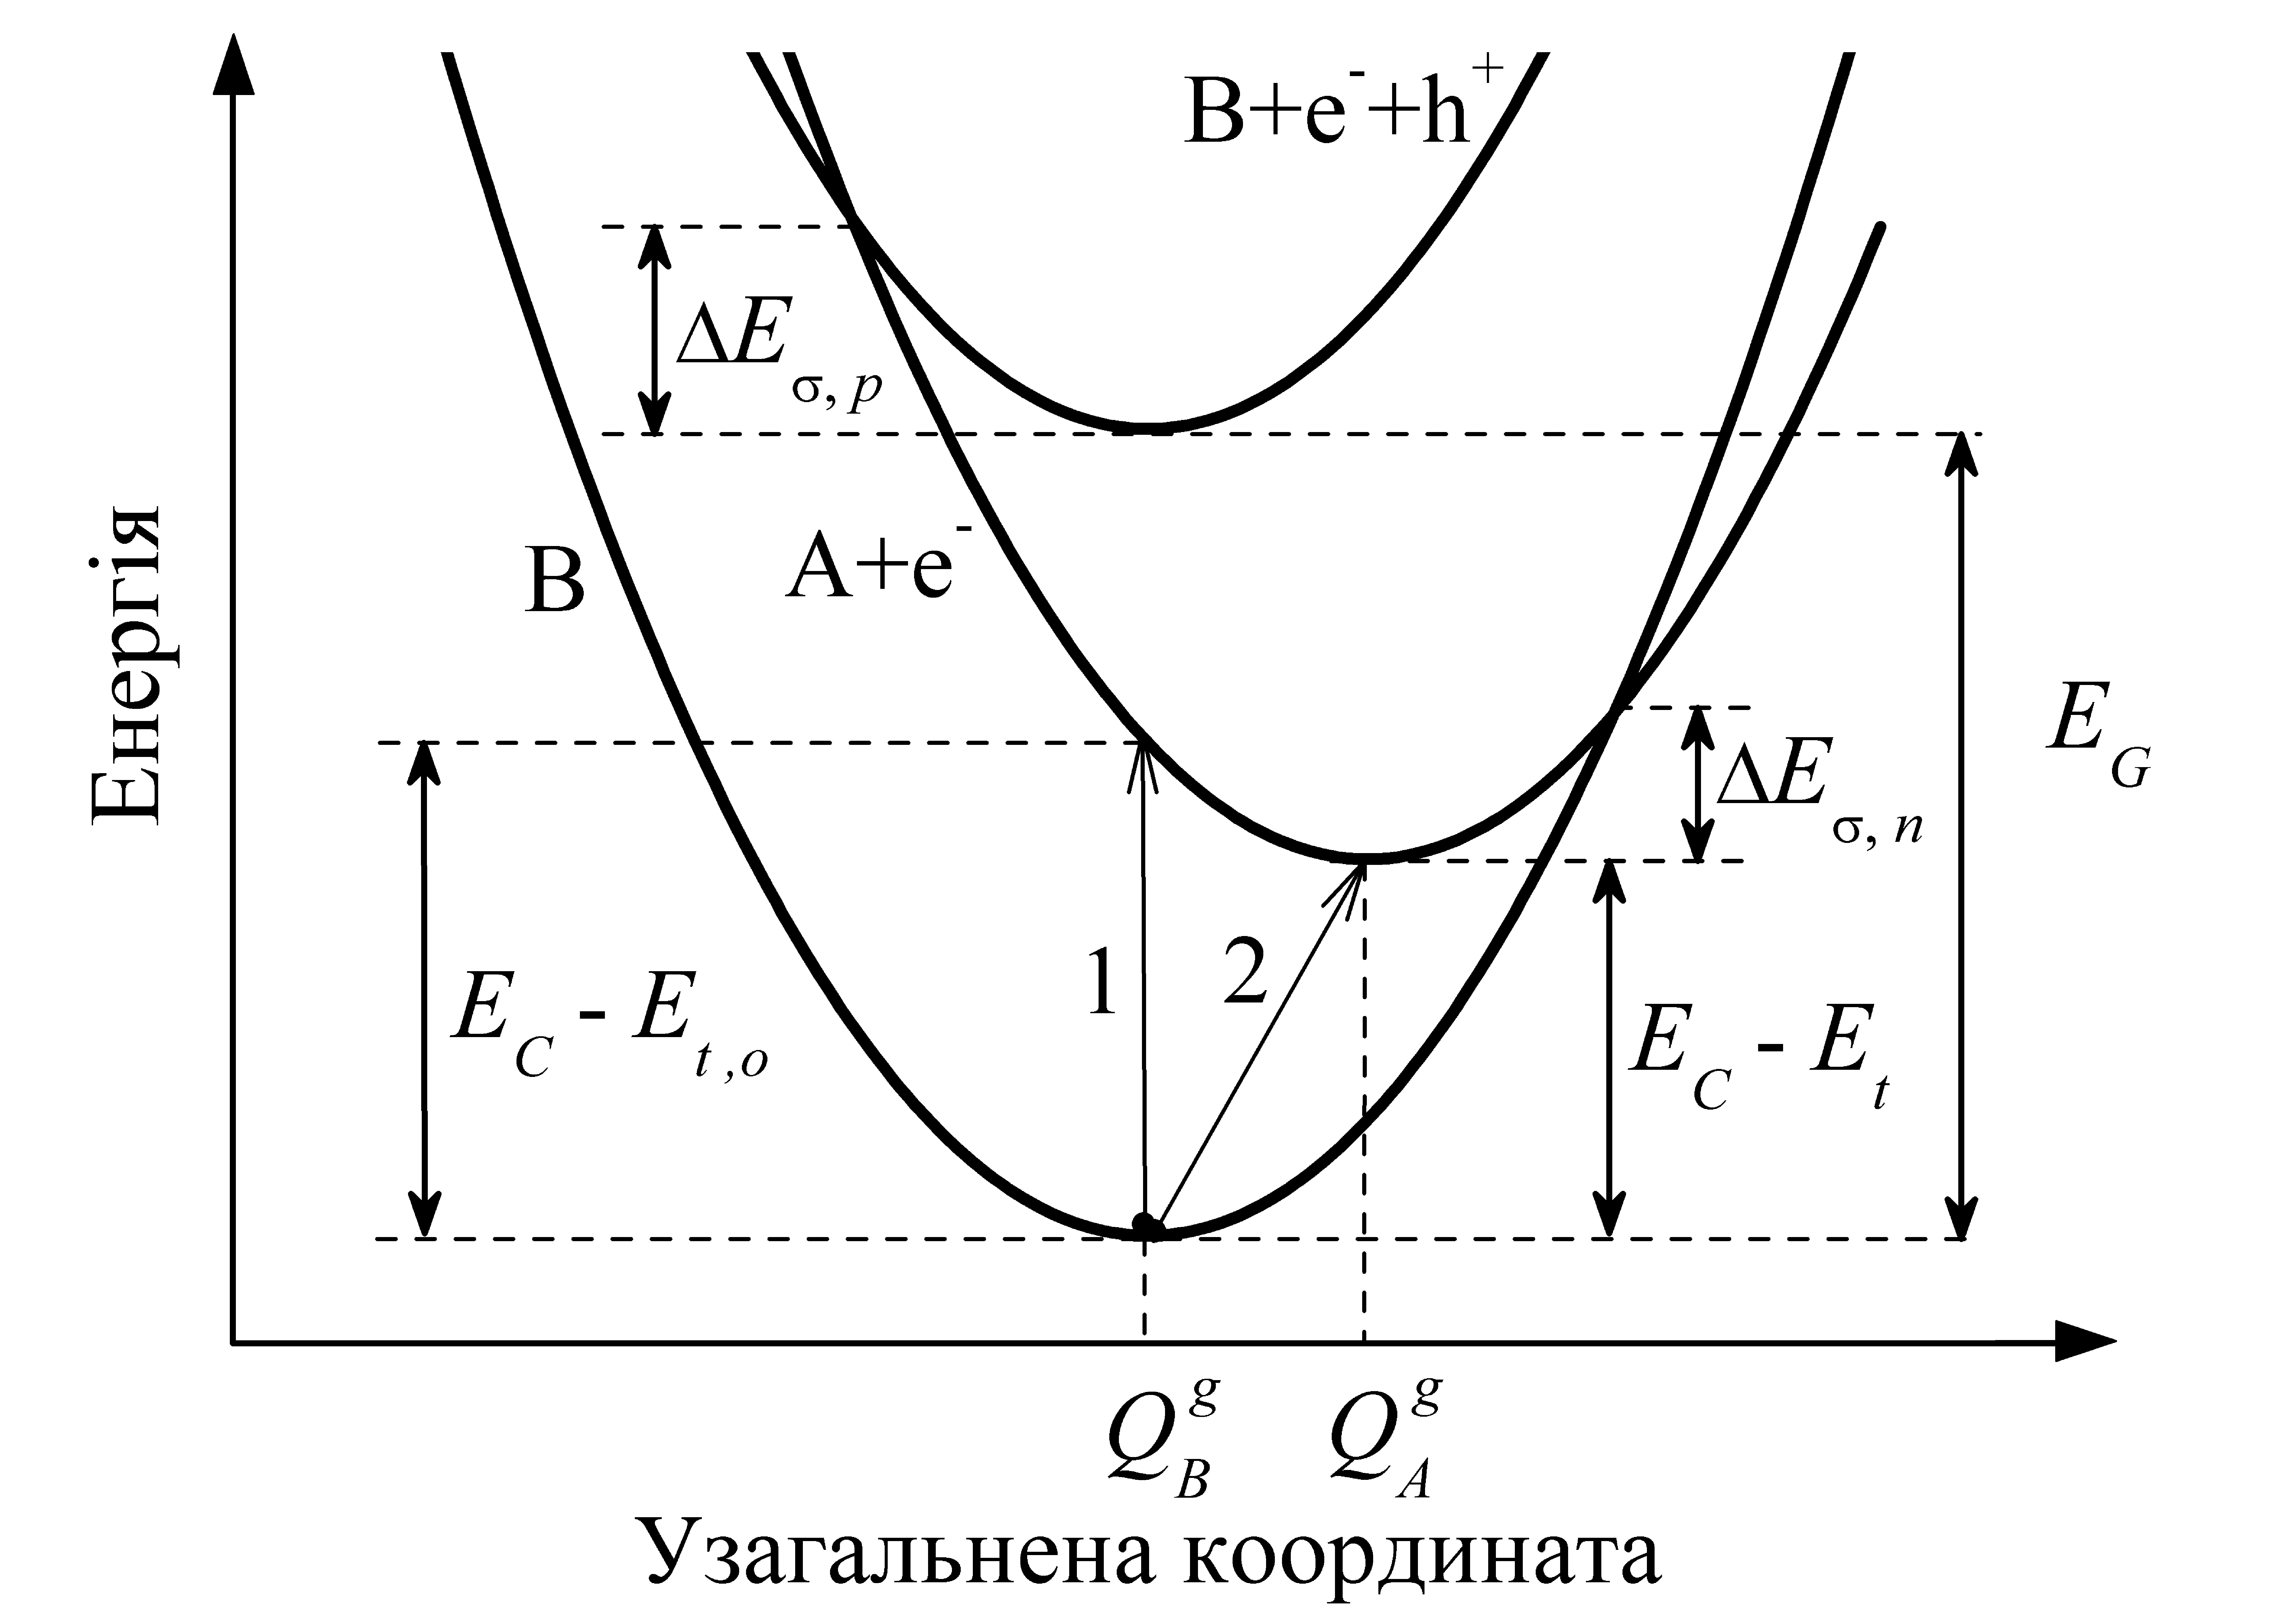
\includegraphics[width=0.7\textwidth]{Fig1_2}
\vspace{-3mm}
\caption{Схематична конфігураційна діаграма для пастки,
розташованій на відстані $E_C-E_{t}$ нижче дна зони провідності.
Нижня парабола відповідає енергії дефекту в стані В,
наступна --- енергії системи (дефект в стані А + вільний електрон),
верхня --- системи (дефект в стані В + вільний електрон + вільна дірка). %\\
Перехід 1 ілюструє оптичну емісію, 2 --- термічну.}
\vspace{-3mm}
\label{F12}
\end{figure}

Подібна ситуація зображена на рис.~\ref{F12},
де припускається, що станам дефекту А та В у рівновазі
відповідають різні узагальнені координати $Q_A^g$ та $Q_B^g\neq Q_A^g$.
Це означає, що при перезарядці дефекту для досягнення рівноваги
має змінитися просторове положення атомів.
Зазвичай ці процеси значно повільніші, ніж електронний перехід
внаслідок поглинання фотона і тому під час фотоіонізації відбуватися не встигають.
Отже, оптично--стимульованій емісії на конфігураційній діаграмі відповідає вертикальний перехід
(1 на рис.~\ref{F12}).
В той же час, під час термічної емісії процес атомної релаксації  відбувається і тому
такий перехід на конфігураційній діаграмі має позначатися прямою, яка з'єднує мінімуми ---
перехід 2 на рис.~\ref{F12}.

Таким чином, оптичний рівень $E_{t,o}(n_e/n_e+1)$ асоціюється
з переходом між зарядовими станами (А та В), проте енергія кінцевого
стану має розраховуватися для атомної конфігурації початкового стану.
Оптичний рівень визначається, наприклад, у методах абсорбційної спектроскопії,
фотолюмінесценції, катодолюмінесценції, тобто коли у кінцевому
зарядовому стані не відбувається релаксація до рівноважної конфігурації.
Термічний рівень $E_{t}(n_e/n_e+1)$ може бути означений як положення рівня Фермі,
при якому стани А та В мають однакову енергію і при цьому у кінцевому після електронного переходу стані
мають повністю відбутися релаксаційні процеси.
Рівні такого типу спостерігаються в дослідженнях перехідної спектроскопії,
термостимульованих струмів, температуро-залежних холівських вимірюваннях тощо.

Зауважимо, що на рис.~\ref{F12} також показані термоактиваційні енергії поперечних перерізів захоплення
заряду при багатофононному захопленні.




\chapter{Метод перехідної спектроскопії \\ локальних рівнів}\label{chapDLTS}
%\section{Еволюція комп'ютерних мереж}\label{sec101}

У 1974~р. Д.Ланг запропонував елегантний метод визначення параметрів дефектів дефектів,
який базується на вимірюваннях релаксації ємності бар'єрних структур після прикладання
імпульсу напруги \cite{Lang} .
Метод отримав назву перехідної спектроскопії локальних рівнів (deep--level transient spectroscopy, DLTS).
Фізичною передумовою методу є той факт, що ширина області просторового заряду в структурах Шотки чи $p$--$n$--переходах
залежить від прикладеної напруги, а отже змінюючи цю величину можна керувати положенням рівня Фермі в певному
прошарку матеріалу.

Розглянемо для визначеності контакт електронного напівпровідника з металом.
На рис.\ref{F21} представлена схема енергетичної діаграми такої структури при двох значеннях зворотної напруги $V$.
Поблизу межі розділу в напівпровіднику розташовується  збіднений шар,
тобто область зі зменшеною кількістю вільних носіїв заряду, яка виникла
внаслідок присутності електричного поля.
Її ширина визначається з умови
\begin{equation}
W=\left[\frac{2\varepsilon\varepsilon_0(V_{bi}+V)}{q^2N_D}\right]^{0.5}\,,
\end{equation}
де
$\varepsilon$ --- діелектрична проникність напівпровідника,
$\varepsilon_0$ ---діелектрична стала,
$V_{bi}$ --- контактна різниця потенціалів,
%$V$ ---прикладена до контакту зворотна напруга,
$N_D$ --- концентрація донорів,
$q$ --- елементарний заряд.

\begin{figure}[t]
\center
\vspace{-5mm}
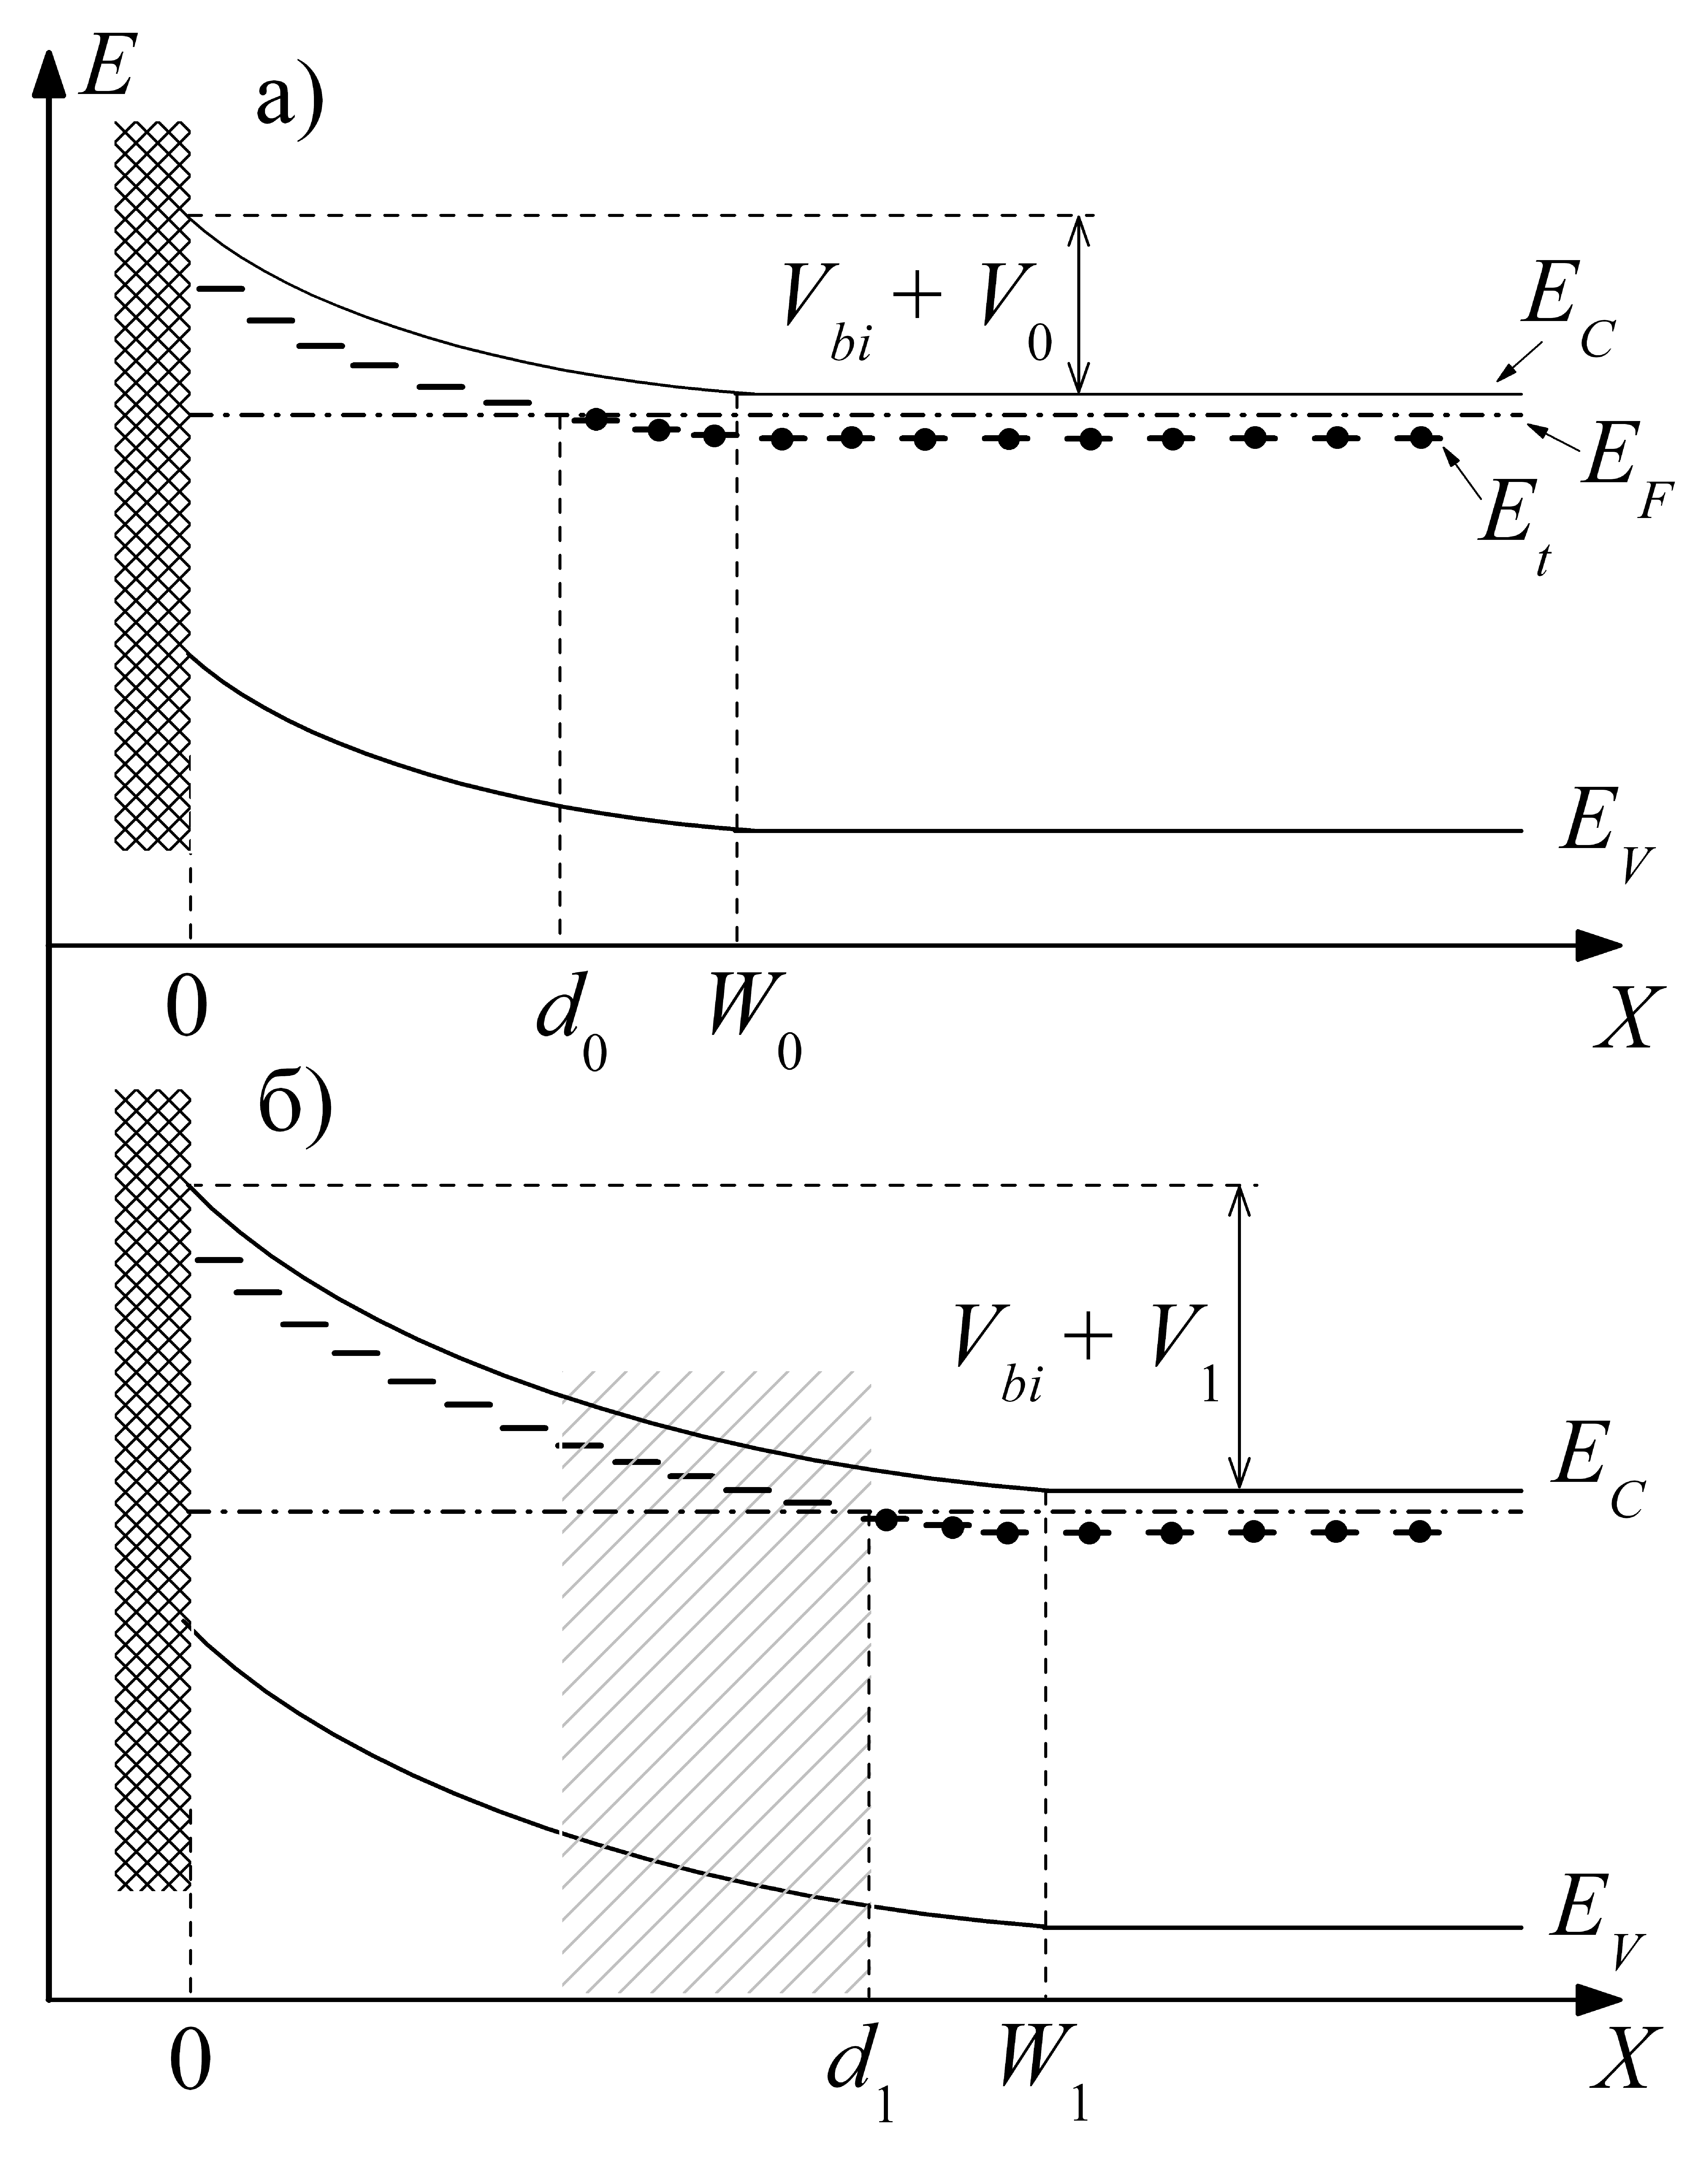
\includegraphics[width=0.6\textwidth]{Fig2_1}
\vspace{-3mm}
\caption{Зонна діаграма контакту Шотки при
різних значення зворотної напруги $V_0$ (а) та $V_1$ (б).
Вважається, що в області $x<0$ розташовано метал,
а при  $x>0$ --- $n$--напівпровідник.
$V_{bi}$ --- контактна різниця потенціалів,
$W_0$ та $W_1$ --- ширини області просторового заряду,
$d_0$ та $d_1$ --- координати межі між областями різного зарядового
стану дефекту.
}
\vspace{-3mm}
\label{F21}
\end{figure}

Припустимо, що у напівпровіднику є рівномірно розподілений по об'єму дефект з концентрацією $N_t$ , якому
відповідає глибокий рівень $E_t$.
Якщо в глибині напівпровідника $E_F>E_t$, а $(V_{bi}+V)>(E_C-E_t)$,
то в збідненому шарі буде проходити межа між  областями, де дефект перебуває у різних зарядових станах.
Відстань цієї межі від контакту можна оцінити за допомогою співвідношення
\begin{equation}
d=W-\left[\frac{2\varepsilon\varepsilon_0(E_F-E_t)}{q\,N_D}\right]^{0.5}=W-\lambda_d\,.
\end{equation}
Якщо звернутися до рис.\ref{F21}, то при $x>d$
рівень буде переважно заповненим, при $x<d$ --- вільним.

У збідненому шарі присутній просторовий заряд $Q$, викликаний в загальному випадку
як іонізованими донорними домішками
(вже нескомпенсованими вільними електронами, як це відбувається в глибині напівпровідника)
так і зарядженими дефектами.
Величина заряду залежить від прикладеної напруги і тому розглядають таке поняття як диференційна
ємність структури:
\begin{equation}
\label{DLTSC}
C=\frac{dQ}{dV}\,.
\end{equation}
У випадку, коли концентрація дефектів достатньо низька та їхнім внеском у $Q$ можна знехтувати
\begin{equation}
\label{DLTSCsh}
C=A\left[\frac{q\varepsilon\varepsilon_0\,N_D}{2(V_{bi}+V)}\right]^{0.5}\,,
\end{equation}
де
$A$ --- площа структури.

При зміні величини зворотної напруги (напр., від $V_0$ до $V_1$,
як це показано на рис.~\ref{F21},а та \ref{F21},б відповідно),
повинні зміститися як межа збідненого шару (від $W_0$ до $W_1$),
так межа розділу областей з різним зарядовим станом дефекту (від $d_0$ до $d_1$).
Якщо перший процес визначається перерозподілом
вільних носіїв заряду і відбувається достатньо швидко (за час порядку максвелівського часу релаксації),
то для реалізації другого необхідно, щоб всі дефекти, розташовані в прошарку
між $d_0$ та $d_1$ емітували електрони.
Цей процес значно повільніший і тому безпосередньо після зміни напруги
в системі може бути зафіксована ємність $\Delta C$ надлишкова, порівняно з рівноважним випадком, що
описується виразом (\ref{DLTSCsh}).
У випадку низької концентрації дефектів ($\Delta C\ll C$), а також за умови $(W_1-W_0)\ll W_1$,
цю величину можна оцінити за допомогою співвідношення \cite{tuomisto2019}
\begin{equation}
\label{DLTdelC}
\Delta C=\frac{N_t\,C_0}{2N_D}\left[1-\frac{2\lambda_d}{W}\left(1-\frac{C(V)}{C_0}\right)-\left(\frac{C(V)}{C_0}\right)^2\right]\,,
\end{equation}
де
$C_0=C(0)$.
При $C_0\gg C(V)$ вираз спрощується
\begin{equation}
%\renewcommand{\theequation}{\thechapter.\arabic{equation}*}
%\addtocounter{equation}{-1}
\label{DLTdelC*}
\Delta C=\frac{N_t\,C_0}{2N_D} \,,\tag{\ref{DLTdelC}\,$'$}
\end{equation}

%\begin{equation}
%\label{DLTSint}
%\int_{d_0}^{d_1}\frac{dC}{C}=-\int_{d_0}^{d_1}\frac{n(x)}{N_D\,W^2}x \,dx\,.
%\end{equation}

\begin{figure}[b]
\center
\vspace{-5mm}
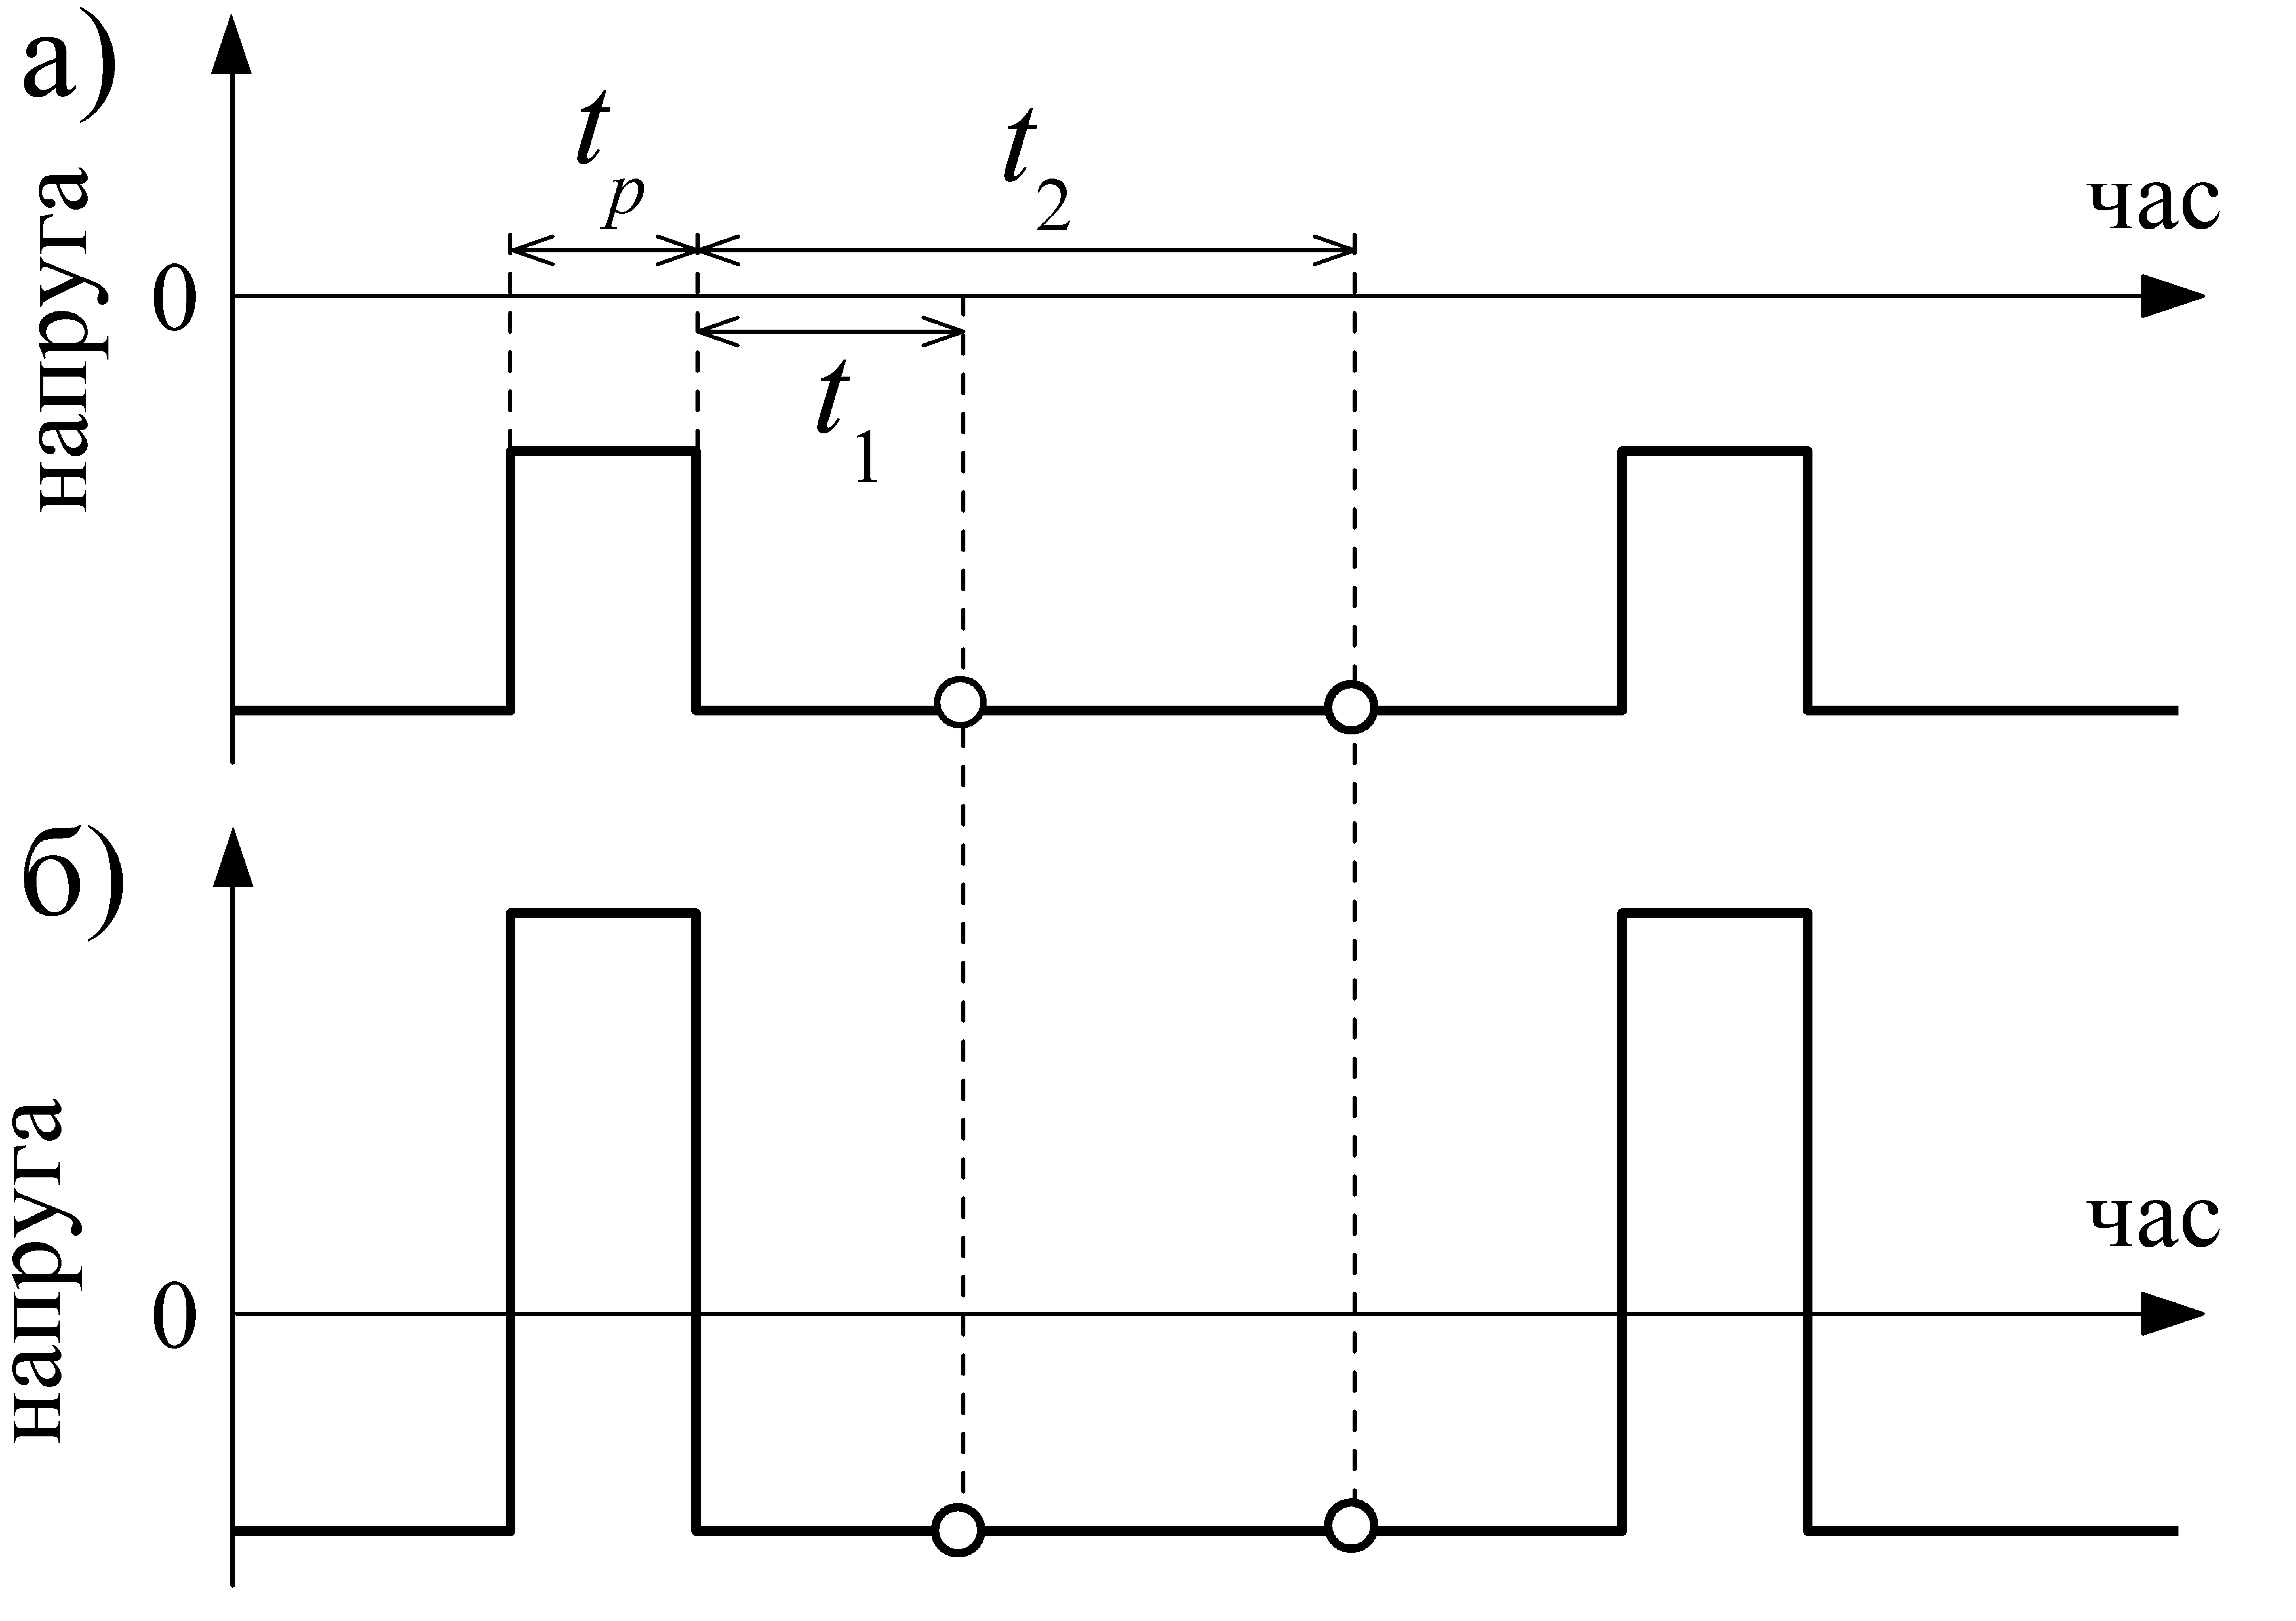
\includegraphics[width=0.6\textwidth]{Fig2_2}
\vspace{-3mm}
\caption{Режими зміщення бар'єрної структури в метод DLTS.
Кружечками позначено моменти виміру ємності.
}
\vspace{-3mm}
\label{F22}
\end{figure}


\begin{figure}[ht]
\center
\vspace{-5mm}
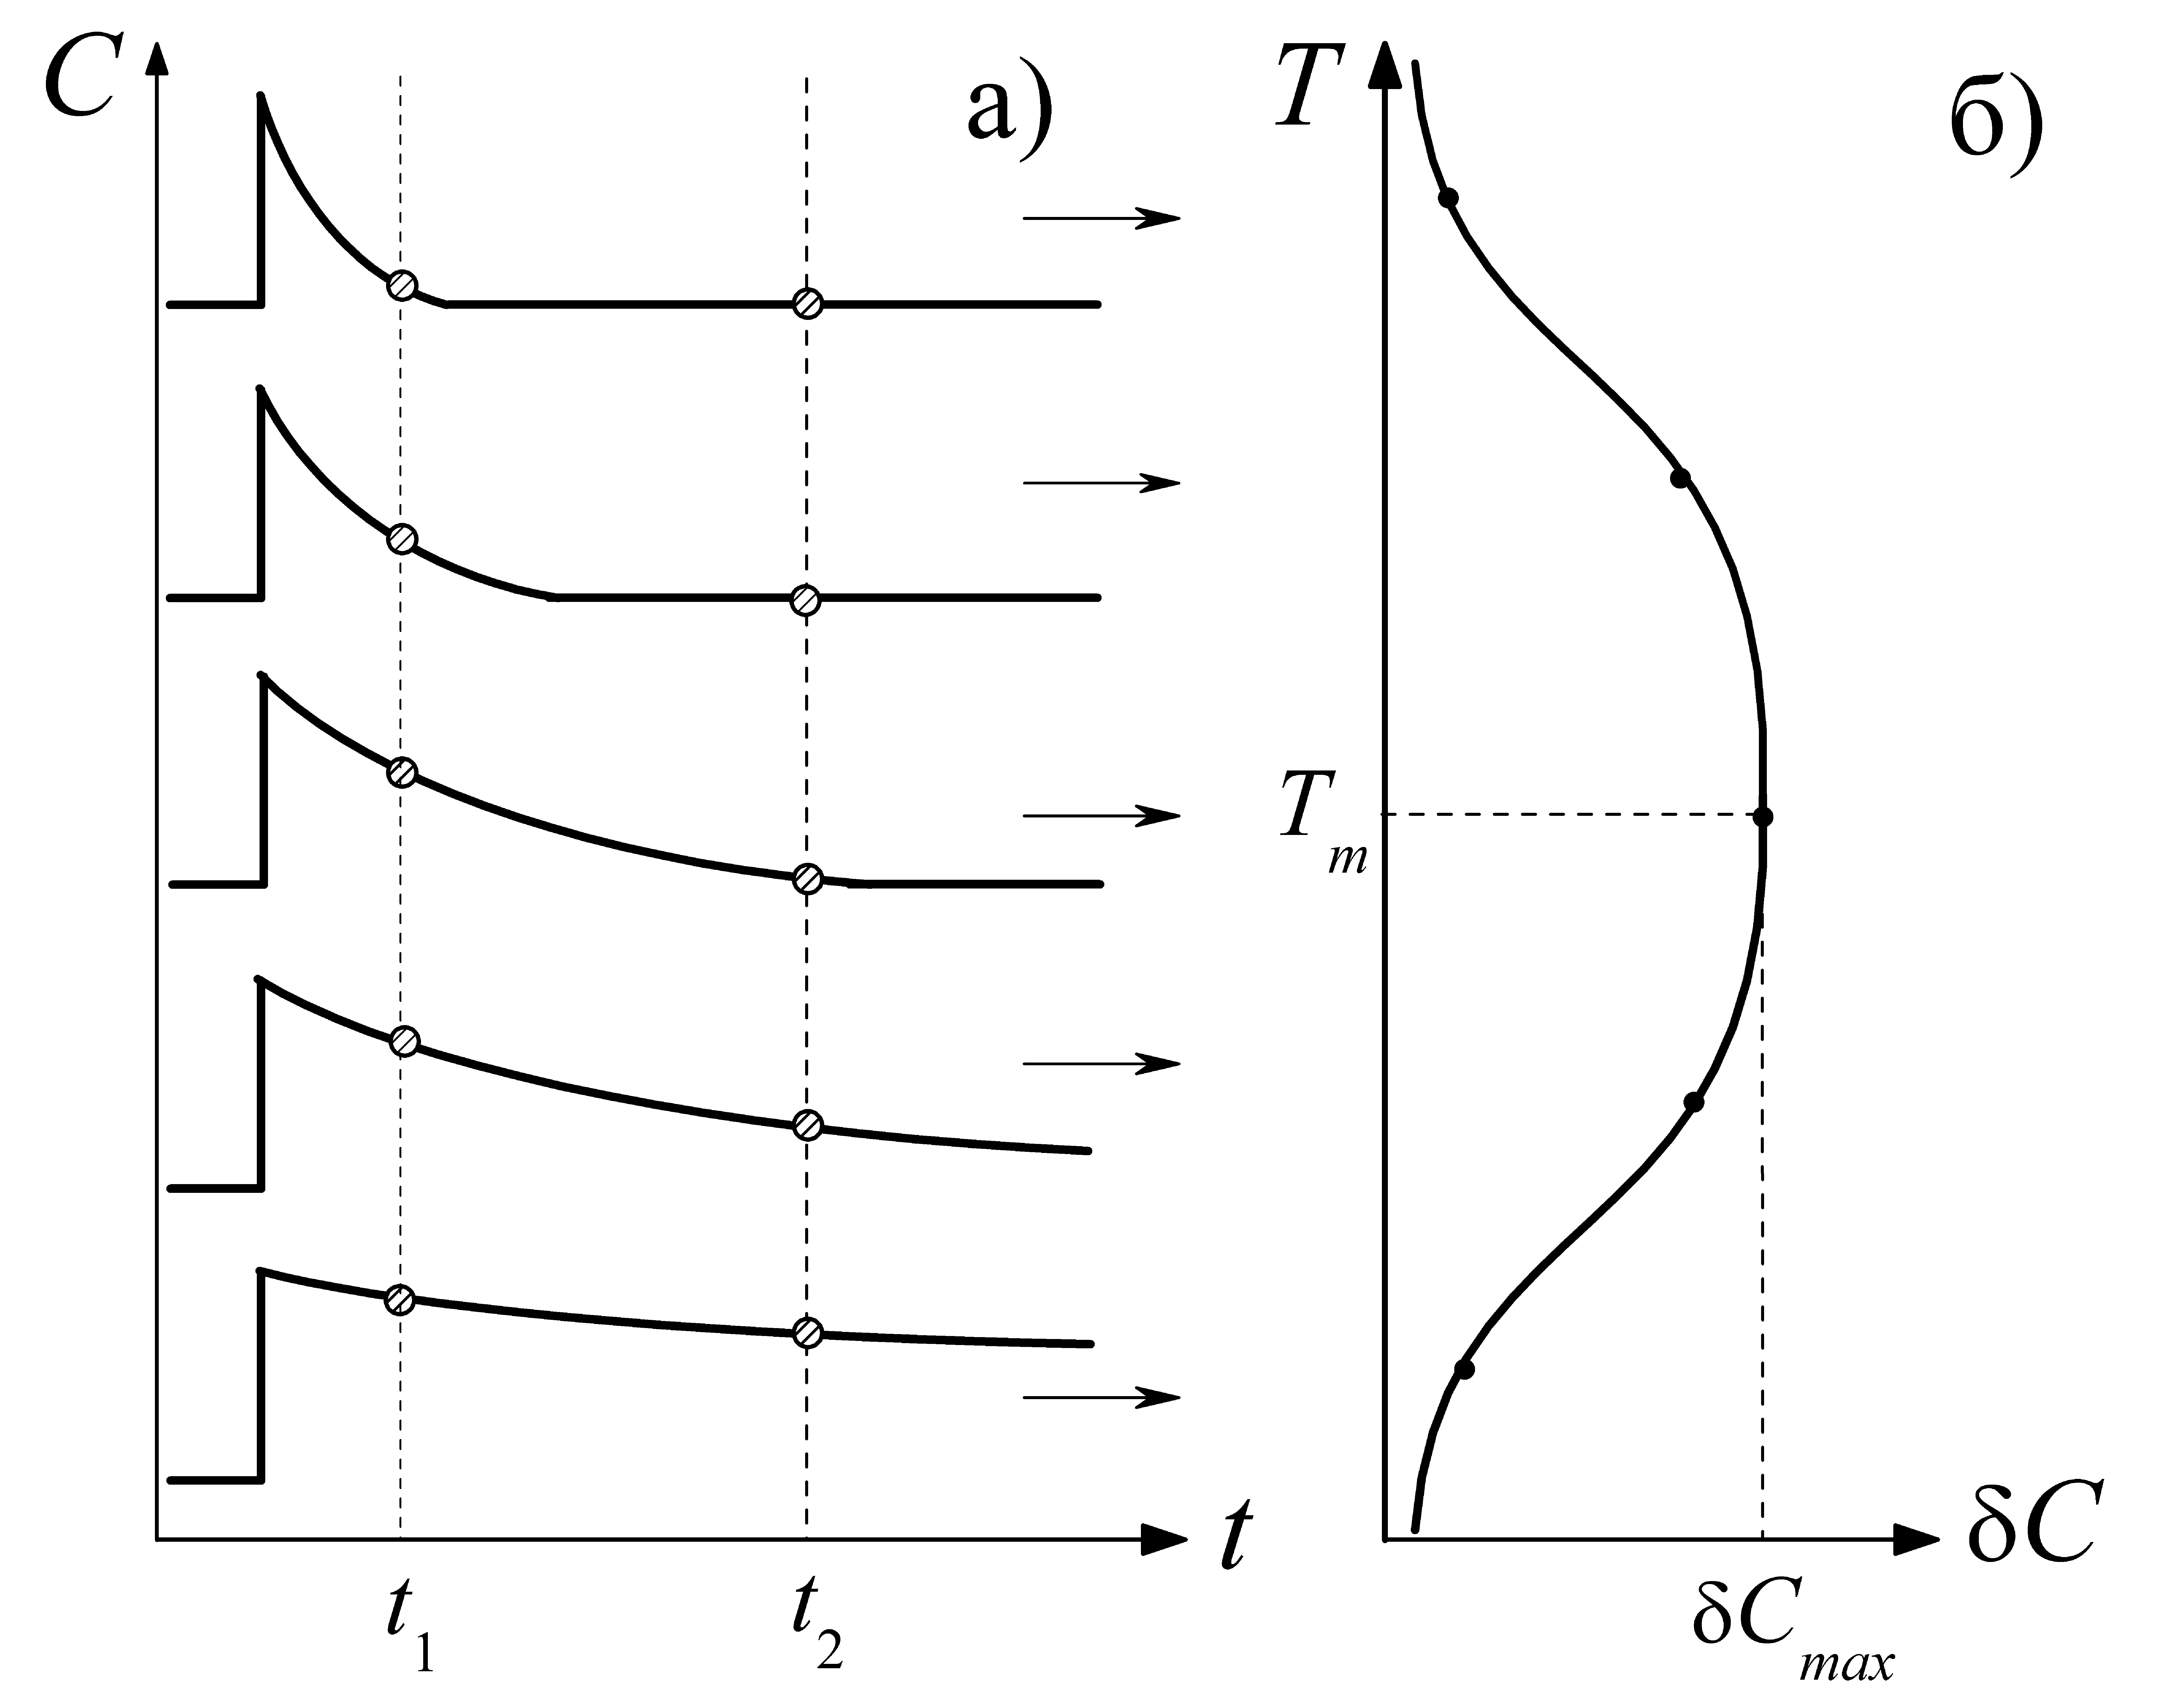
\includegraphics[width=0.65\textwidth]{Fig2_3}
\vspace{-3mm}
\caption{(а)~Характер релаксації ємності при різних температурах;
(б)~Спектр DLTS.
}
\vspace{-3mm}
\label{F23}
\end{figure}




Зазвичай напругу прикладають у імпульсному режимі, наприклад як показано на рис.\ref{F22},
вимірюючи ємність після закінчення так званого імпульсу заповнення тривалістю $t_p$
у два різних моменти часу ($t_1$ та $t_2$ на рисунку).
Саме різниця $\delta C=C(t_1)-C(t_2)$ і є сигналом DLTS.
Кінетика зміни ємності визначається процесом перезарядки дефектів
та за умов, зазначених вище, описується експоненційною залежністю:
\begin{equation}
\label{DLTSdelC}
C(t_1)-C(t_2)=\Delta C\,\left[\exp(-e_n t_1)-\exp(-e_n t_2)\right]\,,
\end{equation}
де
$e_n$ визначається виразом (\ref{en}).
Вимірювання проводяться в певному температурному діапазоні, залежність
$\delta C$ від температури називається спектром DLTS.
Швидкість емісії зростає з підвищення температури,
проте як при повільній (при низькій температурі) релаксації,
так і швидкі (при високій)
значення ємності в моменти вимірювання відрізняються мало --- див. рис.~\ref{F23},а.
Тому залежність $\delta C(T)$
характеризується наявністю максимуму (рис.~\ref{F23},б)
Відповідне екстремуму $\delta C(T)$ значення $e_{n,max}$ можна знайти з умови
\begin{equation*}
\left.\frac{d(\delta C)}{d e_n}\right|_{e_n=e_{n,max}}=0\,.
\end{equation*}
Враховуючи (\ref{DLTSdelC}), отримуємо
\begin{gather}
% \nonumber to remove numbering (before each equation)
  \frac{d\delta C}{d e_n} = \Delta C \left[-t_1\exp(-e_n t_1)+t_2\exp(-e_n t_2)\right]\,, \nonumber\\
  t_2\exp(-e_{n,max} t_2)-t_1\exp(-e_{n,max} t_1)= 0\,,\nonumber\\
  t_2\exp(-e_{n,max} t_2)= t_1\exp(-e_{n,max} t_1)\,, \nonumber\\
  \frac{t_2}{t_1} = \exp(-e_{n,max} (t_2-t_1))\,, \nonumber\\
  e_{n,max}=\frac{\ln\left(t_2/t_1\right)}{t_2-t_1}\,.\label{DLTSemax}
\end{gather}
Отже, якщо максимум залежності $\delta C(T)$ спостерігається при температурі $T_m$,
то має виконуватися рівність
\begin{equation}
\label{DLTSTmax}
\sigma_n(T_m)\,\upsilon_{th,n}\gamma_g N_C \exp\left(-\frac{E_C-E_t}{kT_m}\right)=\frac{\ln\left(t_2/t_1\right)}{t_2-t_1}\,.
\end{equation}

\begin{figure}[!b]
\center
\vspace{-5mm}
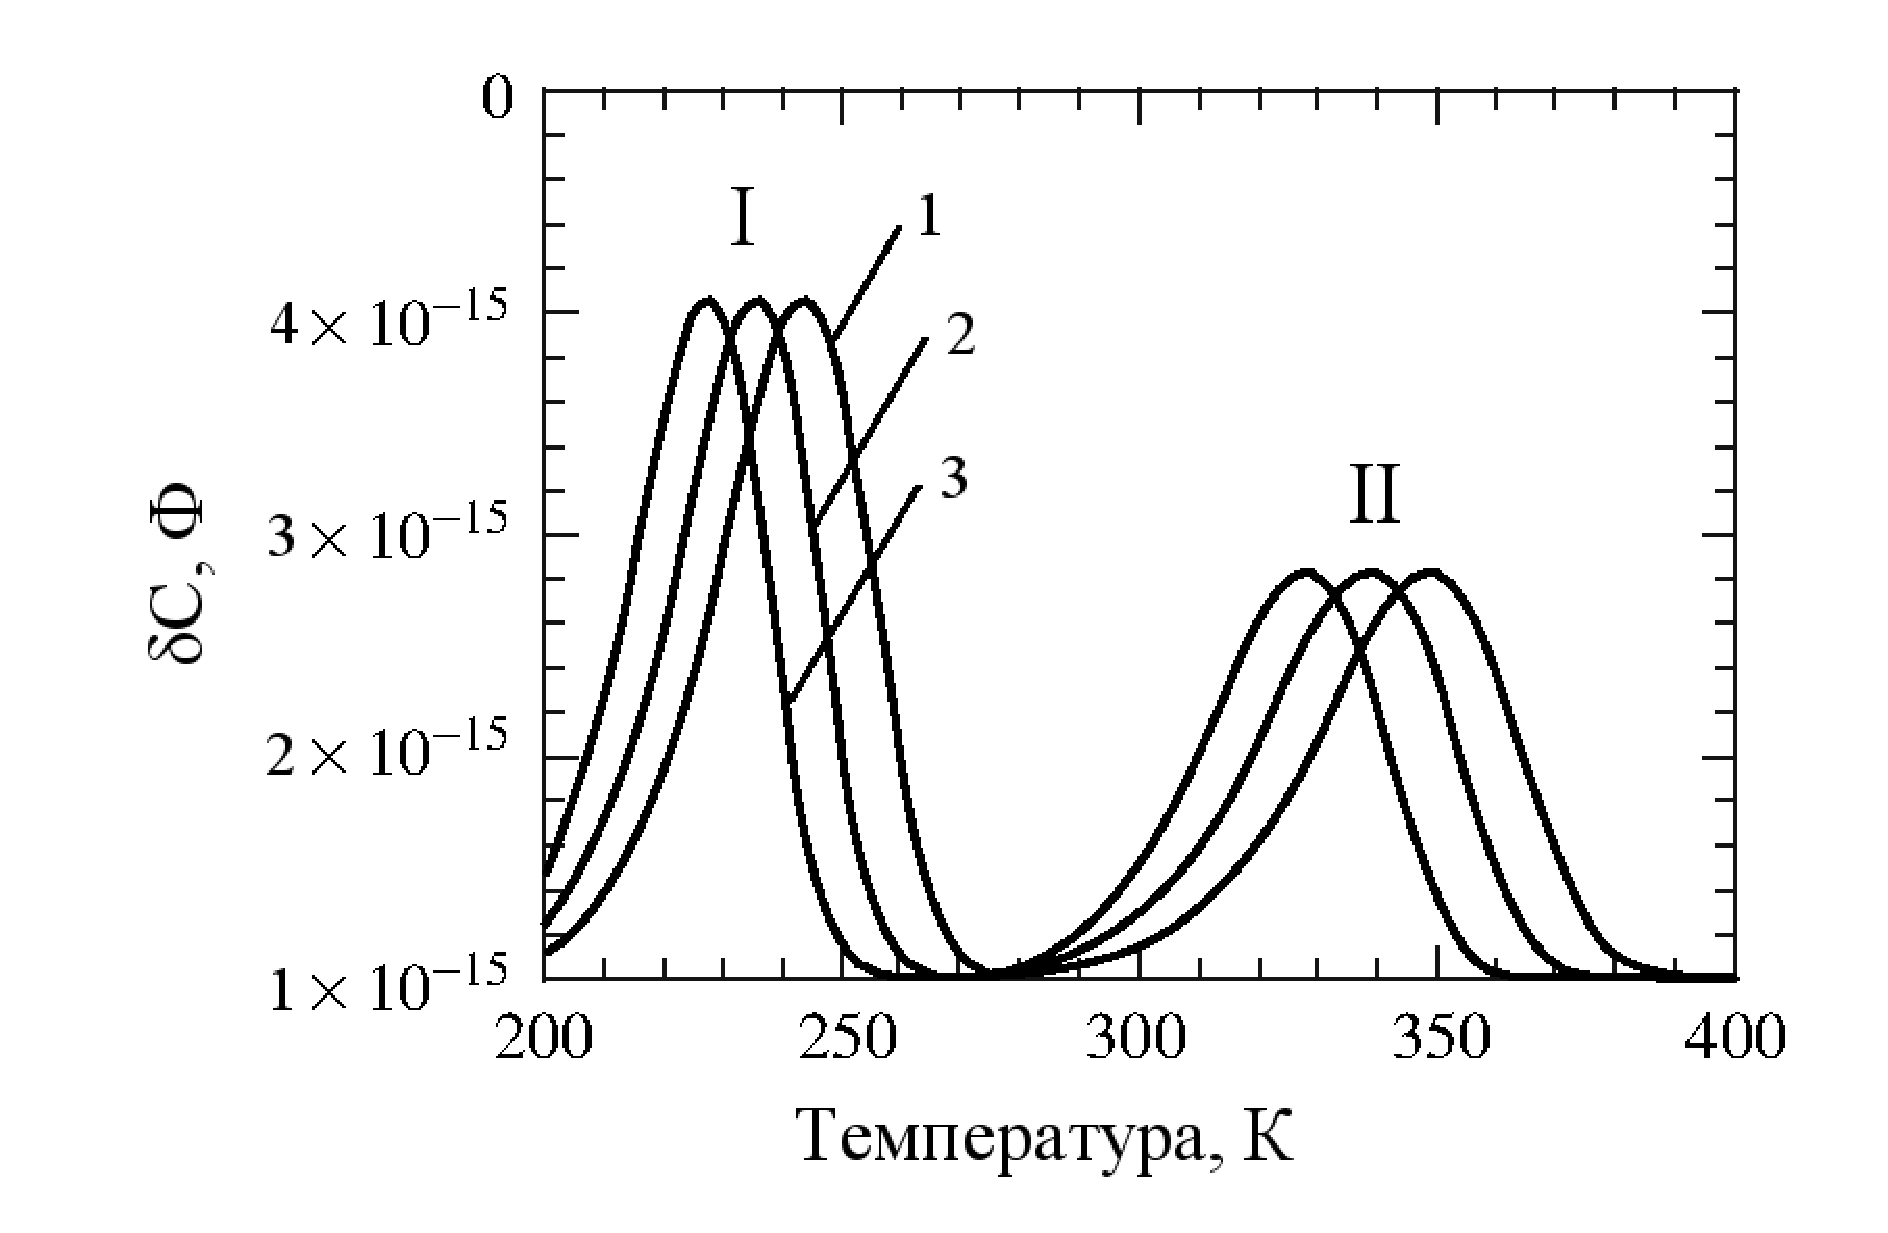
\includegraphics[width=0.65\textwidth]{Fig2_4}
\vspace{-3mm}
\caption{Розраховані спектри DLTS для різних значень $t_1$ та $t_2$.
Були використані значення
$t_1$, мс: 0,5 (крива 1), 1 (2), 2 (3);
$t_1$, мс: 1 (1), 2 (2), 4 (3);
$E_C-E_t$, еВ: 0,37 (для піку I), 0,6 (II);
$\sigma_n$, см$^2$: $10^{-15}$ (I), $5\cdot10^{-15}$ (II);
$N_t$, см$^{-3}$: $5\cdot10^{12}$ (I), $2\cdot10^{12}$ (II);
$C_0=4,9\cdot10^{-12}$~Ф, $N_d=10^{15}$~см$^{-3}$.
Рисунок адаптовано з \cite{Schroder2006}.
}
\vspace{-3mm}
\label{F24}
\end{figure}


Зрозуміло, що однієї рівності (\ref{DLTSTmax}) недостатньо,
щоб визначити дві невідомих характеристики дефекту $E_t$ та $\sigma_n(T_m)$.
Проте можна виміряти спектр DLTS при інших значеннях $t_1$ та $t_2$,
що призведе до зміщення положення максимуму --- відповідний випадок проілюстровано рисунком \ref{F24}.
Як наслідок, експериментально отримується набір температур $\left\{T_{m}\right\}$,
кожній з яких відповідає своя пара з набору  $\left\{(t_{1},t_{2})\right\}$.
Врахувавши співвідношення (\ref{enT}), можемо записати
\begin{equation}
\label{DLTSenT}
\ln\left(\frac{e_{n,max}}{T_m^2}\right)=\ln\left[\frac{\ln\left(t_2/t_1\right)}{\left(t_2-t_1\right)T_m^2}\right]=\ln\left(\beta\sigma_n\right)-\frac{E_C-E_t}{kT_m}\,.
\end{equation}
Тобто залежність $\ln(e_{n,max}\cdot T_m^{-2})$ від оберненої температури має бути прямою лінією,
нахил якої визначається положенням рівня у забороненій зоні, а точка перетину з вертикальною віссю ---
величиною поперечного перерізу захоплення.
Відхилення від лінійності та спотворення отриманих результатів може бути зумовлено температурною залежністю
$\sigma_n$, проте якщо її характер відомий, то цей ефект може бути враховано шляхом введення певних поправок.
Наприклад, якщо поперечний переріз захоплення є термоактивованою величиною (див.~(\ref{Sta})),
то нахил вказаної залежності буде дорівнюватиме не $(E_C-E_t)/k$, а $(E_C-E_t+E_{\sigma})/k$.




Якщо позначити $\delta C_{max}$ величину сигналу DLTS в максимумі,
то використовуючи вирази (\ref{DLTdelC*}), (\ref{DLTSdelC}) та (\ref{DLTSemax}) отримаємо
\begin{gather*}
% \nonumber to remove numbering (before each equation)
  \delta C_{max}=\frac{N_t\,C_0}{2N_D}\,\left\{\exp\left[-\frac{\ln\left(t_2/t_1\right)}{t_2-t_1}\cdot t_1\right]
     -\exp\left[-\frac{\ln\left(t_2/t_1\right)}{t_2-t_1}\cdot t_2\right]\right\}\,.\nonumber
\end{gather*}
Позначивши $b=t_2/t_1$ матимемо
\begin{gather}
% \nonumber to remove numbering (before each equation)
  \delta C_{max}=\frac{N_t\,C_0}{2N_D}\,\left\{\exp\left[-\frac{\ln\left(b\right)}{b-1}\right]
     -\exp\left[-\frac{\ln\left(b\right)}{1-b^{-1}} \right]\right\}\,,\nonumber\\
  \delta C_{max}=\frac{N_t\,C_0}{2N_D}\,\left\{\exp\left[-\frac{\ln\left(b\right)}{b-1}\right]
     -\exp\left[-\frac{b\ln\left(b\right)}{b-1} \right]\right\}\,,\nonumber\\
  \delta C_{max}=\frac{N_t\,C_0}{2N_D}\,\exp\left[-\frac{\ln\left(b\right)}{b-1}\right]\cdot
  \left\{1 -\left(\exp\left[-\frac{\ln\left(b\right)}{b-1} \right]\right)^{b-1}\right\}\,,\nonumber  \\
  \delta C_{max}=\frac{N_t\,C_0}{2N_D}\,\cdot b^{\frac{1}{1-b}}\cdot
  \left(1-\frac{1}{b}\right)\,,\nonumber     \\
    \delta C_{max}=\frac{N_t\,C_0}{2N_D}\,\cdot b^{\frac{1}{1-b}-1}\cdot \left(b-1\right)
                  =\frac{N_t\,C_0}{2N_D}\,\cdot b^{\frac{b}{1-b}}\cdot \left(b-1\right)\,,\nonumber \\
    N_t=\frac{2N_D\,\delta C_{max}b^{\frac{b}{b-1}}}{C_0\,(b-1)}\,.
\end{gather}
Тобто за висотою максимуму у спектрі DLTS можна  оцінити концентрацію дефектів.

Типова роздільна здатність при DLTS вимірюваннях $\delta C_{max}/C_0\approx(10^{-5}\div 10^{-4})$,
а отже метод дозволяє виявити дефекти з концентрацією порядку $(10^{-5}\div 10^{-4})N_D$.


При нерівномірному розподілі дефектів вираз (\ref{DLTdelC*}) перестає бути справедливим.
Водночас, варіюючи величину імпульсів заповнення та беручи до уваги відносні зміни ємності
можна оцінити профіль концентрації дефектів:
\begin{equation}
\label{DLTSNt}
N_t(x)=\left(\frac{N_D^2W^2q}{\varepsilon\varepsilon_0}\right)\left(\frac{x-\lambda}{x}\right)\frac{d\left(\frac{\Delta C}{C}\right)}{dV}\,.
\end{equation}

Якщо у захопленні носіїв активно приймають участь декілька типів дефектів, то кожному
з них на спектрі DLTS буде відповідати свій пік.
Для випадку, коли параметри дефектів істотно відрізняються, ці піки легко розділяються
і DLTS дозволяє отримати параметри кожного з дефектів.


У вищеописаному традиційному DLTS--методі під час імпульсу заповнення заселеність пасток,
які переважно захоплюють неосновні носії заряду, не змінюється.
А отже, досліджуються рівні, які знаходяться, переважно, лише у одній половині  забороненої зони
(верхній для прикладу, що розглядався).
Але варіюючи знак імпульсів прикладеної до бар'єрної структури напруги можна
проводити дослідження різних типів дефектів, у тому числі й тих, які захоплюють носії заряду протилежних знаків.
Наприклад, для вивчення центрів захоплення неосновних носіїв може бути використаних режим,
ілюстрований рис.~\ref{F22}.
При прямому зміщенні інжектуються як основні, так і неосновні носії заряду та
відбувається зміна ємності збідненого прошарку внаслідок захоплення носіїв
обох знаків.
При наступному зворотному зміщенні процеси захоплення пригнічуються і
захоплені носії звільняються внаслідок термічної емісії.
Причому DLTS спектр у цьому випадку буде визначатися суперпозицією сигналів
від пасток обох типів.
Такий варіант досліджень нерідко називається інжекційна DLTS (inj--DLTS).

\begin{figure}[!b]
\center
\vspace{-5mm}
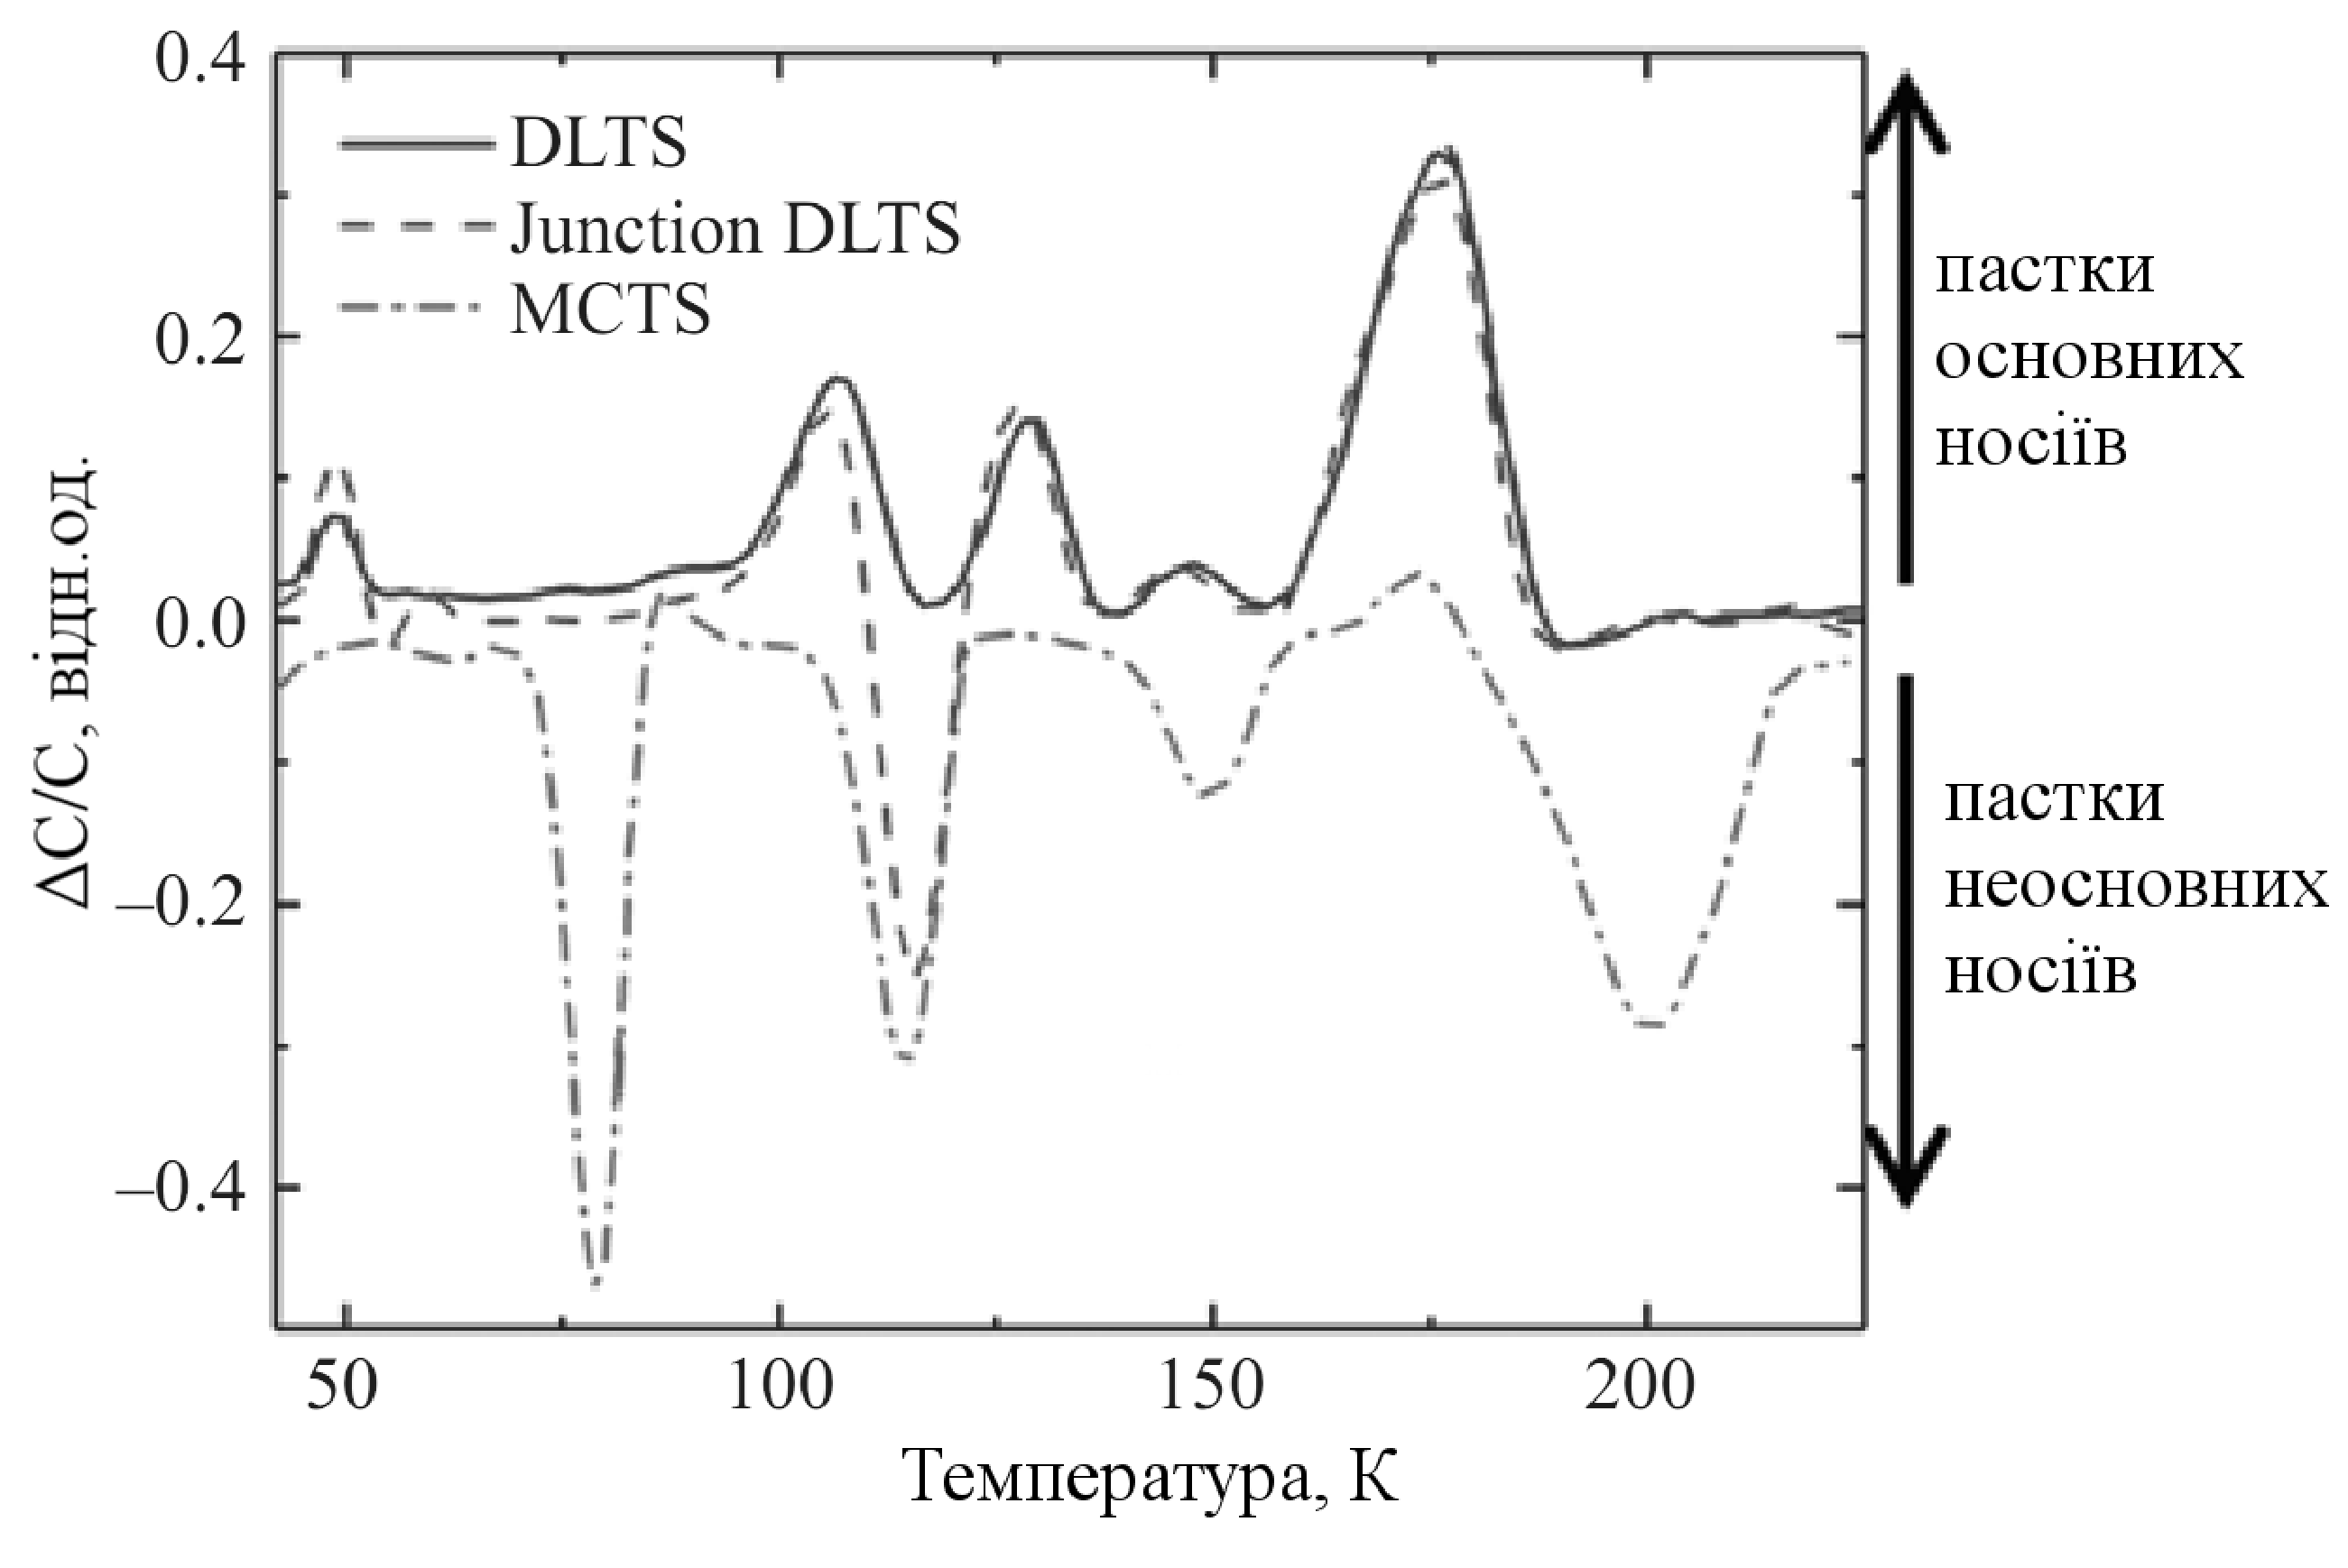
\includegraphics[width=0.75\textwidth]{Fig2_5}
\vspace{-3mm}
\caption{Спектри DLTS, inj--DLTS та MCTS.
Рисунок адаптовано з \cite{tuomisto2019}.
}
\vspace{-3mm}
\label{F25}
\end{figure}

Можна реалізувати випадок, коли в область просторового заряду вводяться лише неосновні носії.
Наприклад, подібна ситуація реалізується  при біполярній генерації носіїв за межами збідненого шару
на відстані порядку довжини дифузії від його межі.
Зокрема, цього можна досягти при освітленні структури з протилежного від бар'єру боку
і наступній дифузії в напрямку фронтальної площини.
Такий варіант DLTS називається MCTS (minority carrier transient spectroscopy).
В цьому випадку релаксація ємності та спектр матимуть протилежний знак.
Як приклад на рис.~\ref{F25} представлені спектри DLTS, інжекційної DLTS та MCTS.


За час застосування методу перехідної спектроскопії з'явилися й інші його модифікації.
Наприклад у методі ODLTS (optical deep--level transient spectroscopy), як і у традиційному DLTS,
вимірюється температурна залежність нестаціонарної ємності, проте стимуляція
процесів перезарядки глибоких центрів відбувається імпульсами світла, а не напруги.
Зазвичай енергія використаних фотонів менша ширини забороненої
зони ($0.5E_G<h\nu<E_G$),
освітлення відбувається при прикладеній зворотній напрузі.
У випадку напівпровідника $n$--типу, це викликає емісію електронів
з діркових пасток.
Після зняття оптичного імпульсу, пастки емітують дірки і спостерігається релаксація ємності.

У методі DLOS (deep--level optical spectroscopy) реєструється не температурний, а оптичний спектр нестаціонарної ємності.
При цьому існує два варіанти:
в методі термічної DLOS дослідження проводять при температурі, коли пастки внаслідок термічної емісії спустошені
і оптичним шляхом відбувається їх заповнення;
при оптичній DLOS використовується фотонно-стимульована емісія при знижених температурах,
коли вона переважає термічну.

Але чи не найцікавіщим варіантом є Laplace--DLTS (LDLTS) \cite{LDLTS2}.
В цьому випадку вимірювання релаксації ємності проводяться при постійній температурі,
після чого чисельно визначається спектр швидкості рекомбінації.
Процедура  подібна до зворотного перетворення Лапласа,
тобто знаходиться розв'язок рівняння
\begin{equation}
\label{DLTSLapl}
f(t)=\int_0^\infty F(s) e^{-st}ds\,.
\end{equation}
де
$f(t)$ --- виміряна часова залежність,
$F(s)$ --- шукана спектральна функція.
З математичної точки зору чи не найефективнішим вважається
метод регуляризації Тіхонова.
Якщо рівні дефектів розташовані дискретно і релаксація описується
однією чи декількома експонентами, то результуючий спектр
має складатися з $\delta$--подібних піків;
для неперервного енергетичного розподілу очікується широкий спектр.

Laplace--DLTS дозволив істотно підвищити роздільну здатність по енергії.
Наприклад, на рис.~\ref{F26} наведено приклад спектрів традиційного DLTS та LDLTS.
Якщо у першому випадку визначити наявність декількох рівнів
практично неможливо, то в другому присутність двох дефектів очевидна.

\begin{figure}[!t]
\center
\vspace{-5mm}
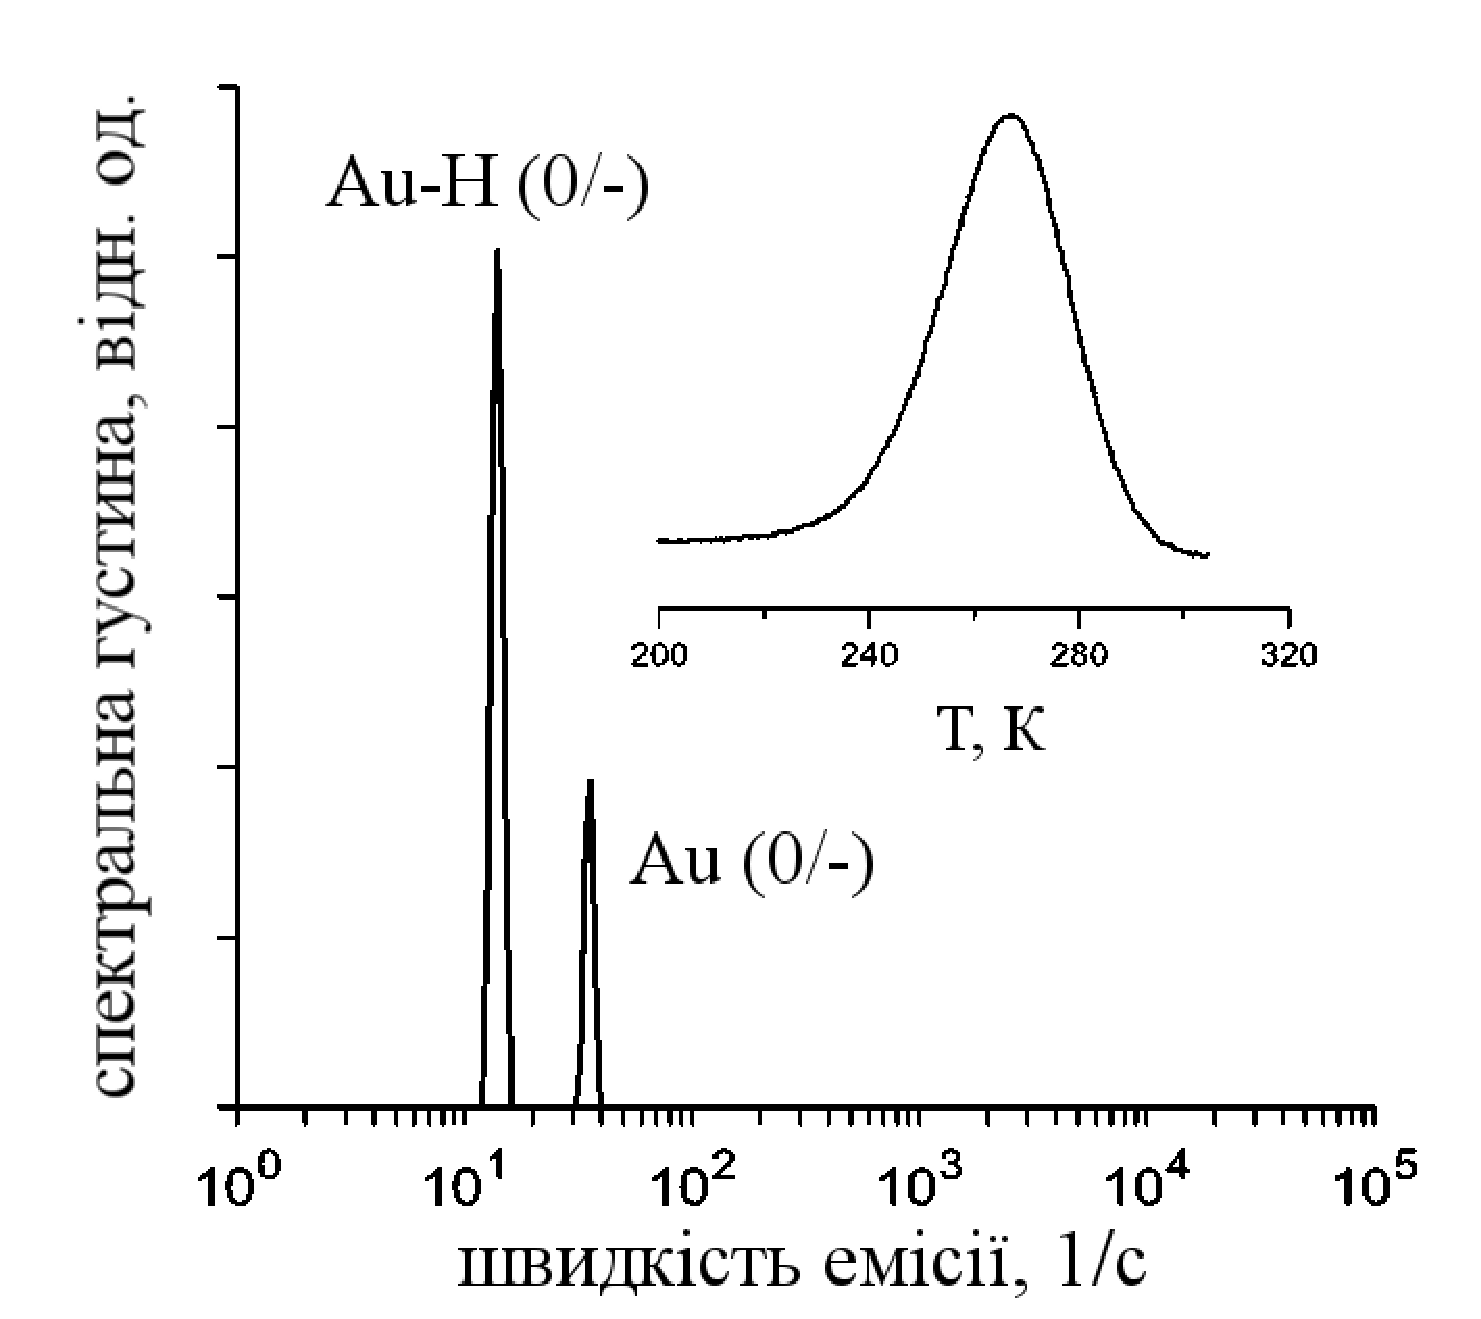
\includegraphics[width=0.65\textwidth]{Fig2_6}
\vspace{-3mm}
\caption{LDLTS спектр Si:(Au,H), виміряний при $T=260$~К.
Піки відповідають акцепторним рівням домішки золота та комплексу
золото--водень.
На вставці --- спектр традиційного DLTS того самого зразка.
Рисунок адаптовано з \cite{Deixler}.
}
\vspace{-3mm}
\label{F26}
\end{figure}

Крім названих варіантів існують й інші, такі як
D--DLTS (double correlation DLTS, використовуються імпульси заповнення з двома різними амплітудами),
СС--DLTS (constant capacitance DLTS, при емісії електронів ємність
залишається постійною завдяки зміні напруги зміщення),
I--DLTS (isothermal DLTS, аналізується похідна ємності по часу, отримана при постійній температурі),
С--DLTS (current DLTS, вимірюється температурна залежність нестаціонарного струму)
тощо.



\chapter{Позитронно--анігіляційна спектроскопія}\label{chapPAS}

Метод позитронно--анігіляційної спектроскопії
(positron annihilation spectroscopy, PAS)
широко почав використовуватися на початку 80--х років XX~ст.,
хоча перші роботи присвячені цьому питання з'явилися на десятиліття раніше.
Як можна здогадатися з назви, у подібних дослідженнях кристал опромінюється позитронами ($\beta^+$--частинками).
При їхній взаємодії з електронами відбувається процес анігіляції
та утворюються два фотони з енергією порядку 511~кеВ,
які рухаються в протилежних напрямках.
Час життя позитронів у кристалі обернено пропорційний електронній густині.
Наявність моменту імпульсу у анігілюючого електрона викликає відхилення
від $180^\circ$ у куті розльоту фотонів та спричинює доплерівський зсув їхньої енергії.
В області розташування дефектів завдяки зміненій електронній густині процеси анігіляції відрізняються від тих,
що відбуваються в ідеальній ґратці і це дозволяє вивчати порушення періодичності.

Основними перевагами цього методу вважаються
\begin{itemize}[leftmargin=0em,itemindent=1.5em]
%\begin{enumerate}[label=\arabic*),leftmargin=0em,itemindent=1.5em]
\item можливість безпосередньої ідентифікації дефектів вакансійного типу та
селективне виявлення подібних дефектів;
\item суттєве теоретичне підґрунтя, що дозволяє, зокрема, розрахувати характеристики анігіляції з перших принципів;
\item застосовність як до об'ємних матеріалів, так і до тонких плівок з будь-якою провідністю.
\end{itemize}

Основними джерелами позитронів у експериментах є:
\begin{enumerate}[label=\asbuk*),leftmargin=0em,itemindent=1.5em]
  \item радіоактивні ізотопи;
  наприклад, достатньо широко використовується ізотоп $^{22}\text{Na}$, для якого характерні наступні реакції
  \begin{gather*}
  ^{22}\text{Na}\rightarrow \:^{22}\text{Ne}^{*}+\beta^++\nu_e\,,\\
  ^{22}\text{Ne}^{*}\rightarrow \:^{22}\text{Ne}+h\nu\,,
  \end{gather*}
де
$\nu_e$ --- нейтрино,
$^{22}\text{Ne}^{*}$ ---збуджений стан ізотопу неону,
друга реакція відбувається через 3 пс після першої і супроводжується
випроміненням $\gamma$--кванту з енергією 1,27~МеВ;
період напіврозпаду цього ізотопу $T_{1/2}=2,6$~роки, що
дозволяє ефективно використовувати одне джерело на протязі 6-10 років;
 типова інтенсивність джерела порядку $10^9$ позитрон/с;
  \item ядерні реактори чи прискорювачі, які характеризуються значно більшою інтенсивністю --- до $10^{12}$ позитрон/с.
\end{enumerate}
В обох випадках енергетичний спектр отриманих позитронів неперервних,
середнє значення енергії близько сотні кеВ (для ізотопу $^{22}\text{Na}$ --- 0,18~МеВ).

Коефіцієнт поглинання позитронів можна оцінити за допомогою співвідношення \cite{PAS}
\begin{equation}
\alpha_+\approx\frac{\varrho\,\left[\text{г}/\text{см}^3\right]}{E_{+,m}^{1/4}\,[\text{МеВ}]}\:\text{см}^{-1}\,,
\end{equation}
де
$\varrho$ --- густина речовини,
$E_{+,m}$ --- максимальна енергія спектру позитронів (для $^{22}\text{Na}$ --- 0,54~МеВ).
Типові глибини проникнення ($\alpha^{-1}_+$) складають близько 110~мкм для Si та 40~мкм для GaN (при використання ізотопного джерела).

При розгляді позитронного опромінення використовують
таку величину як ймовірність поглинання (анігіляції) налітаючої частинки
при проходженні неї у речовині шляху одиничної довжини ($P_L$),
% $[P_L]=\text{см}^{-1}$).
розмірність якої обернено пропорційна відстані.
Залежність $P_L$ від глибини проникнення називається профілем поглинання (stopping profile).
При безпосередньому використанні радіоактивних джерел профіль екпоненційний:
\begin{equation}\label{PASPl1}
P_L(x)=\alpha_+\,\exp(-\alpha_+\,x)\,.
\end{equation}
Вираз (\ref{PASPl1}) записано у припущенні, що
напрям осі $X$ збігається з напрямом поширення позитронів,
а точка $x=0$ відповідає границі матеріалу.
Якщо взяти до уваги величини $\alpha_+$, то очевидно,
що такий режим опромінення придатний лише для дослідження об'ємних
(товщиною декілька сотень мікрометрів) матеріалів.
При характеризації дефектів у тонких плівках позитрони
бажано сповільнити до енергій менше 50кеВ та, за можливості, монохроматизувати.
В цьому випадку
\begin{equation}\label{PASPl2}
P_L(x)=-\frac{d}{dx}\exp\left[-\left(\frac{x}{x_0}\right)^2\right]\,.
\end{equation}
де
$x_0$ --- розташування максимуму профілю поглинання.
При цьому середнє значення глибини проникнення $\bar{x}$  з одного боку
задовольняє умові $\bar{x}\simeq \,0,886\, x_0$ (профіль не симетричний),
а з другого --- визначається енергією позитрону $E_{+}$:
\begin{equation}
\bar{x}=-\frac{4\cdot10^{-6}}{\varrho\left[\text{мкг}/\text{см}^3\right]}\cdot E_{+}^{1,6}\,\text{кеВ}\,.
\end{equation}

У загальному випадку темп анігіляції позитронів $\lambda_+$ описується виразом
\begin{equation}\label{PASL}
\lambda_+=\frac{1}{\tau_+}=\pi\,r_e^2\,c\int\left|\psi_+(\overrightarrow{r})\right|^2\,\rho_e(\overrightarrow{r})\,d\overrightarrow{r}\,.
\end{equation}
де
$\tau_+$ --- час життя позитронів,
$r_e=\frac{q^2}{4\pi\varepsilon_0 m c^2}\approx2,8\cdot10^{-15}\,\text{м}$ --- класичний радіус електрону,
$\psi_+$ --- хвильова функція позитрону,
$\rho_e$ --- електронна густина.
Як видно з (\ref{PASL})  $\lambda_+$ пропорційна перекриттю позитронних та електронних густин.

Позитрони, як і електрони, можуть локалізуватися біля порушень ґратки --- тобто, знаходячись біля дефектів мати енергію,
яка є недозволеною для них у ідеальній ґратці.
При цьому
\begin{enumerate}[label=\asbuk*),leftmargin=0em,itemindent=1.5em]
%\begin{enumerate}[label=\arabic*),leftmargin=0em,itemindent=1.5em]
\item для дефектів вакансійного типу відповідні рівні глибокі, енергія іонізації $E_{t+}\geq$1~еВ;
\item для від'ємно заряджених домішок заміщення та міжвузольних дефектів рівні мілкі,
 енергія зв'язку становить $(10\div100)$~меВ і
непогано описується у наближенні теорії ефективної маси.
%енергія зв'язку становить $10\div100$~меВ, а отже при температурі $100\div300$~К відповідні стані іонізовані.
\end{enumerate}

Швидкість захоплення позитронів дефектом описується виразом
\begin{equation}\label{PASc}
c_+=\frac{N_t\,\mu_t}{\rho_N}\,.
\end{equation}
де
$\rho_N$ --- концентрація ядер,
а коефіцієнт $\mu_t$ залежить як від типу дефекту, так і від властивостей основної ґратки.

Для додатно заряджених як вакансій, так і дефектів іншого типу, значення $\mu_t$
настільки малі, що за час життя позитрону відповідні процеси практично не встигають відбуватися і тому
PAS не здатна виявляти дефекту у такому зарядженому стані.
Для нейтральної вакансії $\mu_t\approx10^{14}\div10^{15}$~c$^{-1}$ і практично не залежить від температури;
для негативно зарядженої $\mu_t\approx10^{15}\div10^{16}$~c$^{-1}$ при $T=300$~K і зростає при
зниженні температури (у спрощеному випаду при врахуванні лише зміни теплової швидкості
позитрону $\mu_t\sim T^{-1/2}$).
Для дефектів, пов'язаних з негативно зарядженими іонами величина $\mu_t$ приблизно така ж сама
як для V$^-$.
Проте необхідно врахувати, що відповідно до принципу детальної рівноваги
\begin{equation}\label{PASce}
\frac{e_+}{c_+}=\frac{1}{N_t}\left(\frac{m_+^*kT}{2\pi\hbar^2}\right)^{3/2}\exp\left(-\frac{E_{t+}}{kT}\right)\,,
\end{equation}
де
$e_+$ --- швидкість емісії позитронів,
$m_+^*$ --- ефективна маса позитрону, як правило $m_+^*\approx1,5 m_0$.
А отже, для мілких рівнів анігіляція захоплених позитронів може спостерігатися лише при
$T<100$~К, при вищих температурах вони термічно іонізовані.
В той же час для вакансій $e_+\approx0$.

Припустимо, що
$p_{b}^+(t)$ --- частка вільних позитронів у кристалі в момент часу $t$ відносно до загальної початкової кількості позитронів, а
$p_{t,j}^+(t)$  --- частка позитронів, захоплених дефектами $j$--го типу.
Тоді систему рівнянь, яка описує кінетику зміни кількості позитронів можна записати у вигляді
\begin{equation}\label{PASdin}
\left\{
\begin{aligned}%{rl}
\frac{dp_{b}^+(t)}{dt}=& -\lambda_{+,b} \:p_{b}^+ - \sum_j c_{+,j} \:p_{b}^+ + \sum_j e_{+,j} \,p_{t,j}^+ \,,\\
\frac{dp_{t,j}^+(t)}{dt}=& c_{+,j} \:p_{b}^+ - \lambda_{+,tj}\,p_{t,j}^+ - e_{+,j} \,p_{t,j}^+ \,,
\end{aligned} \right.
\end{equation}
де
$\lambda_{+,b}$ та $\lambda_{+,tj}$ описують темп анігіляції позитронів, які знаходяться
у об'ємі кристалу та які захоплені дефектом $j$--го  типу.
Вважається, що у початковий момент часу $p_{b}^+(0)=1$, $p_{t,j}^+(0)=0$ --- всі позитрони вільні.

Наприклад, якщо у кристалі присутні один дефект вакансійного типу
(характеризується параметрами $\lambda_{+,\mathrm{V}}$, $c_{+,\mathrm{V}}$ та $e_{+,\mathrm{V}}\approx0$)
та один дефект, що є причиною появи мілкого позитронного рівня з параметрами
$\lambda_{+,\mathrm{ST}}$, $c_{+,\mathrm{ST}}$ та $e_{+,\mathrm{ST}}$ (<<ST>> --- shallow trap),
то система рівнянь виглядатиме наступним чином
\begin{equation}\label{PASdin2}
\left\{
\begin{aligned}%{rl}
\frac{dp_{b}^+}{dt}=& -(\lambda_{+,b}+c_{+,\mathrm{V}}+c_{+,\mathrm{ST}}) \:p_{b}^+ +e_{+,\mathrm{ST}}\,p_{\mathrm{ST}}^+ \,,\\
\frac{dp_{\mathrm{V}}^+}{dt}=& c_{+,\mathrm{V}} \:p_{b}^+ - \lambda_{+,\mathrm{V}}\,p_{\mathrm{V}}^+ \,,\\
\frac{dp_{\mathrm{ST}}^+}{dt}=& c_{+,\mathrm{ST}} \:p_{b}^+ - (\lambda_{+,\mathrm{ST}}+e_{+,\mathrm{ST}})\,p_{\mathrm{ST}}^+ \,.
\end{aligned} \right.\tag{\ref{PASdin}\,$'$}
\end{equation}
Сумарна частка електронів, які ще не проанігілювали у момент часу $t$
(ймовірність, що позитрон у цей момент часу ще існує) описується виразом
\begin{equation}\label{PASn1}
p^+(t)=dp_{b}^+(t) + p_{\mathrm{V}}^+(t) + p_{\mathrm{ST}}^+(t)\,.
\end{equation}
Після розв'язку системи рівнянь (\ref{PASdin2}) вираз (\ref{PASn1})  можна
переписати у вигляді
\begin{equation}\label{PASn2}
p^+(t)=\sum_{i=1}^3I_i\exp\left(-\frac{t}{\tau_i}\right)\,,\tag{\ref{PASn1}\,$'$}
\end{equation}
де
$I_i$ та $\tau_i$ будуть залежать від $\{\lambda_{+,b},\lambda_{+,\mathrm{V}},\lambda_{+,\mathrm{ST}},c_{+,\mathrm{V}},c_{+,\mathrm{ST}},e_{+,\mathrm{ST}}\}$,
а також $\sum I_i=1$.

Взагалі, у PAS існує два основних підходи до визначення стану дефектів ---позитронна спектроскопія часу життя
та спектроскопія доплерівського уширення.
Розглянемо їх детальніше.

\section{Позитронна спектроскопія часу життя}\label{secPAS_PSLT}
У цьому варіанті PAS дослідження, як правило, проводять з використанням ізотопного натрієвого джерела,
причому воно використовується у формі NaCl і зберігається у вигляді водного розчину.
У експерименті джерело розміщується між двома ідентичними зразками
(утворюється сандвіч--подібна структура) і
вимірюється проміжок часу між двома подіями:
\begin{itemize}[leftmargin=0em,itemindent=1.5em]
\item появою $\gamma$--фотона з енергією 1,2745~МеВ, що є свідченням появи позитрона і відповідає переходу ізотопу неону зі збудженого стану;
\item появою фотона (або двох) з енергією 0,511~МеВ, яка пов'язана з анігіляцією.
\end{itemize}
У даному випадку спектром є гістограма кількості анігіляційних подій залежно від проміжку часу.
Приклад відповідної залежності наведено на рис.,а.
Після реєстрації враховується наявність фонового шуму та анігіляцію у джерелі --- рис.,б.
Надалі визначається кількість компонент у спадній ділянці.
У найпростішому випадку це можна зробити за кількістю лінійних ділянок на логарифмічній залежності
кількості подій від часу.
Так, для кривої 1 на рис.,б. спостерігається одна така ділянка,
для кривої 2 --- дві.
Після цього отримані дані апроксимуються виразом, подібним (\ref{PASn2}) і визначаються параметри $\{I_i\}$ та $\{\tau_i\}$.
Зокрема, для кривої 2 має бути використана формула
\begin{equation*}
p^+(t)=I_1\exp\left(-\frac{t}{\tau_1}\right)+I_2\exp\left(-\frac{t}{\tau_2}\right)\,,
\end{equation*}
і визначені величини $I_1$, $I_2$, $\tau_1$ та $\tau_2$.
У загальному випадку кількість доданків у сумі також є параметром апроксимації.

Зв'язок визначених величин з параметрами дефектів залежить від можливих шляхів анігіляції позитронів.
Наприклад, крива 2 на рис.,б. свідчить про два можливих механізми зникнення позитронів --- при зустрічі з електронами
у недеформованій ґратці та поблизу дефектів вакансійного типу і
тому рівняння, що описують кінетику анігіляції, виглядатимуть наступним чином:
\begin{gather}
 \frac{dp_{b}^+(t)}{dt}= -\lambda_{+,b}\:p_{b}^+ - c_{+,\mathrm{V}} \:p_{b}^+ \,, \label{PASnb1}\\
\frac{dp_{\mathrm{V}}^+(t)}{dt}= - \lambda_{+,\mathrm{V}}\,p_{\mathrm{V}}^+ + c_{+,\mathrm{V}} \:p_{b}^+ \,.\label{PASnv1}
\end{gather}
Якщо б компонент у спадній ділянці було б більше, то система рівнянь мала б бути складнішою,
але в нашому ілюстративному випадку обмежимося лише наявністю одного вакансійного дефекту.
Тим паче, що на практиці така ситуація спостерігається доволі часто.

У рівнянні (\ref{PASnb1}) змінні розділяються і тому його розв'язок отримати досить просто
\begin{equation}\label{PASnb2}
p_{b}^+(t)=p_{b}^+(0)\exp\left[-(\lambda_{+,b}+c_{+,\mathrm{V}})\,t\,\right]=\exp\left(-\frac{t}{\tau_1}\right)\,,
\end{equation}
тобто $\tau_1^{-1}=\lambda_{+,b}+c_{+,\mathrm{V}}=\tau_{+,b}^{-1}+c_{+,\mathrm{V}}$,
де $\tau_{+,b}$ --- час життя позитронів у ідеальній ґратці.
У виразі (\ref{PASnb2}) враховано, що в початковий момент часу всі позитрони вільні.
Отже, рівняння зміни кількості захоплених дефектом позитронів неоднорідне
\begin{equation}\label{PASnv2}
\frac{dp_{\mathrm{V}}^+(t)}{dt}+\lambda_{+,\mathrm{V}}\,p_{\mathrm{V}}^+=c_{+,\mathrm{V}}\:\exp\left(-\frac{t}{\tau_1}\right)\,.
\end{equation}
Розв'язок однорідного рівняння має вигляд
\begin{equation}
p_{\mathrm{V},\mbox{одн}}^+(t)=p_{\mathrm{V}0}^+\exp\left(-\lambda_{+,\mathrm{V}}\,t\right)
  =p_{\mathrm{V}0}^+\:\exp\left(-\frac{t}{\tau_2}\right)\,,
\end{equation}
де $\tau_2=\lambda_{+,\mathrm{V}}^{-1}=\tau_{+,\mathrm{V}}$ --- час життя позитрону в околі вакансійного дефекту.
Частковий розв'язок неоднорідного рівняння шукатимемо у вигляді
\begin{equation}
p_{\mathrm{V},\mbox{неодн}}^+(t)=A\exp\left(-\frac{t}{\tau_1}\right)\,,
\end{equation}
де величину константи $A$ можна отримати шляхом підстановки останнього виразу у (\ref{PASnv2}):
\begin{gather*}
-\frac{A}{\tau_1}\exp\left(-\frac{t}{\tau_1}\right)+\lambda_{+,\mathrm{V}}A\exp\left(-\frac{t}{\tau_1}\right)=c_{+,\mathrm{V}}\:\exp\left(-\frac{t}{\tau_1}\right)\,,\\
A=\frac{c_{+,\mathrm{V}}}{\lambda_{+,\mathrm{V}}-\tau_1^{-1}}= \frac{c_{+,\mathrm{V}}}{\tau_{+,\mathrm{V}}^{-1}-\tau_{+,b}^{-1}-c_{+,\mathrm{V}}}
=\frac{c_{+,\mathrm{V}}}{\tau_2^{-1}-\tau_1^{-1}}\,.
\end{gather*}
Тобто, загальний розв'язок має вигляд
\begin{equation}\label{PASnb3}
p_{\mathrm{V}}^+(t)=p_{\mathrm{V}0}^+\:\exp\left(-\frac{t}{\tau_2}\right)+\frac{c_{+,\mathrm{V}}}{\tau_2^{-1}-\tau_1^{-1}}\exp\left(-\frac{t}{\tau_1}\right)\,.
\end{equation}
Враховуючи,
що $p_{\mathrm{V}}^+(0)=0$, отримуємо
\begin{equation}\label{PASnb4}
p_{\mathrm{V}0}^+=\frac{c_{+,\mathrm{V}}}{\tau_1^{-1}-\tau_2^{-1}}\,.
\end{equation}
Взявши до уваги вирази (\ref{PASnv2}), (\ref{PASnb3}) та (\ref{PASnb4}),
загальний вираз для кінетики зміни кількості позитронів може бути записаний у вигляді
\begin{equation}\label{PASnRez}
p_{b}^+(t)
%=p_{b}^+(t)+p_{\mathrm{V}}^+(t)
=\exp\left(-\frac{t}{\tau_1}\right)
         +\frac{c_{+,\mathrm{V}}}{\tau_1^{-1}-\tau_2^{-1}}\left[\exp\left(-\frac{t}{\tau_2}\right)-\exp\left(-\frac{t}{\tau_1}\right)\right]\,.
\end{equation}
Відповідно, система співвідношень між експериментально визначеними параметрами
та характеристиками позитронної анігіляції буде наступною
\begin{equation}\label{PASsist}
\left\{
\begin{aligned}
 I_2=&  \,\frac{c_{+,\mathrm{V}}}{c_{+,\mathrm{V}}-\lambda_{+,\mathrm{V}}+\lambda_{+,b}}\,,\\
I_1=& \,1-I_2 \,,\\
\tau_2=&\,\lambda_{+,\mathrm{V}}^{-1}\,,\\
\tau_1=&\,(\lambda_{+,b}+c_{+,\mathrm{V}})^{-1}\,.
\end{aligned} \right.
\end{equation}

Для визначення величини $\lambda_{+,b}=\tau_{+,b}^{-1}$ можна використати
опорний зразок з того самого матеріалу, де відсутнє вакансійне захоплення і сигнал складається лише з однієї
експоненційної компоненти.
Зауважимо, що $\tau_{+,b}$ слабко залежить від рівня легування напівпровідника і може слугувати
табличною характеристикою матеріалу.
Наприклад, для кремнію $\tau_{+,b}\approx221$~пс.



\begin{table}[bth]
\caption {Час життя позитронів в околі вакансіних кластерів у кремнії}
\label{tabltau} %\center{
%\begin{tabular}{|p{0.18\textwidth}|*{5}{p{0.14\textwidth}|}}
\begin{tabularx}{\textwidth}{|>{\centering\arraybackslash}X|>{\centering\arraybackslash}X|>{\centering\arraybackslash}X|>{\centering\arraybackslash}X|>{\centering\arraybackslash}X|>{\centering\arraybackslash}X|}
  \hline
  дефект & V&V$_2$ &V$_3$&V$_4$&V$_5$    \tabularnewline \hline
  $\tau_{+,\mathrm{V}}$, пс & 254&299&321&330&355   \tabularnewline \hline
\end{tabularx}
%\end{tabular}
%}
\end{table}

Спираючись на визначену величину $c_{+,\mathrm{V}}$ та теоретичну розраховану $\mu_\mathrm{V}$ можна,
за допомогою виразу (\ref{PASc}), оцінити концентрацію вакансій.

Якщо проводити вимірювання при різних температурах, то
за відсутністю (чи наявністю) температурної залежності $c_{+,\mathrm{V}}$ можна зробити
висновок про нейтральність (чи негативний заряд) вакансійного дефекту;
Крім того, як вже зазначалося вище, величини $\tau_{+,\mathrm{V}}$ та $c_{+,\mathrm{V}}$ залежать від зарядового стану
вакансії, який, в свою чергу, визначається положенням рівня Фермі, що також змінюється з температурою.
Наприклад, для напівпровідника з електронною провідністю
\begin{equation}\label{EF}
E_F(T)=\frac{1}{2}(E_D+E_C)-\frac{1}{2}kT\ln\left(\frac{N_C(T)}{\gamma_{g,D}N_D}\right)\,,
\end{equation}
де
$E_D$ --- енергетичний рівень, пов'язаний з донорною домішкою,
$\gamma_{g,D}$ --- фактор його виродження.
Якщо положення рівня вакансії $E_{t}$ таке, що
в досліджуваному температурному діапазоні змінюється його розташування
відносно $E_F$, то на температурних залежностях $\tau_{+,\mathrm{V}}$ та $c_{+,\mathrm{V}}$
має спостерігатися злам --- див. рис., намальований для випадку рівня  $E_t(0/-)$.
При цьому розташування зламу ($T_{br}$) дозволяє визначити розташування рівня дефекту
\begin{equation}
E_t =E_F(T_{br})\,.
\end{equation}

В позитронній спектроскопії часу життя можна також розглядати
парціальні анігіляції в різних станах $\eta_+$.
Наприклад,
для системи з двома механізмами анігіляції
розглядати $\eta_{+,b}$ та $\eta_{+,\mathrm{V}}$ ---
частки позитронів, які анігілювали у ґратці та в околі вакансійних
дефектів, відповідно;
у більш загальному випадку говорити про $\eta_{+,b}$ та $\{\eta_{+,tj}\}$.
Зауважимо, що $\eta_{+,b}+\eta_{+,\mathrm{V}}=1$ 
(або $\eta_{+,b}+\sum_j\eta_{+,tj}=1$).
Тоді середній час життя позитронів $\left\langle\tau_+\right\rangle$
з одного боку буде визначати виразом
\begin{equation*}
\left\langle\tau_+\right\rangle=\eta_{+,b}\tau_{+,b}+\eta_{+,\mathrm{V}}\tau_{+,\mathrm{V}}\,.
\end{equation*}
а з іншого
\begin{equation*}
\left\langle\tau_+\right\rangle=I_1\tau_{1}+I_2\tau_{2}\,.
\end{equation*}
З цього, зокрема, випливає, що
\begin{equation*}
\eta_{+,b}=\frac{\lambda_{+,b}}{\lambda_{+,b}+c_{+,\mathrm{V}}}\,;\quad
\eta_{+,\mathrm{V}}=\frac{c_{+,\mathrm{V}}}{\lambda_{+,b}+c_{+,\mathrm{V}}}\,.
\end{equation*}

$\left\langle\tau_+\right\rangle$ взагалі може бути ключовим параметром,
який безпосередньо визначається з експериментальних залежностей.
Наприклад, коефіцієнт захоплення позитронів дефектом можна визначити саме через цю величину
\begin{equation*}
c_{+,\mathrm{V}}=\frac{1}{\tau_{+,b}}\,\cdot\,\frac{\left\langle\tau_+\right\rangle-\tau_{+,b}}{\tau_{+,\mathrm{V}}-\left\langle\tau_+\right\rangle}\,.
\end{equation*}



 % {}^{22}\text{Na}\rightarrow ^{22}\text{Ne^*}+\beta^++\nu_e


%\end{gather}

\bibliography{defMethodLit}
\addcontentsline{toc}{chapter}{\bibname}



\end{document}
